\documentclass[12pt,]{article}
\usepackage{lmodern}
\usepackage{amssymb,amsmath}
\usepackage{ifxetex,ifluatex}
\usepackage{fixltx2e} % provides \textsubscript
\ifnum 0\ifxetex 1\fi\ifluatex 1\fi=0 % if pdftex
  \usepackage[T1]{fontenc}
  \usepackage[utf8]{inputenc}
\else % if luatex or xelatex
  \ifxetex
    \usepackage{mathspec}
  \else
    \usepackage{fontspec}
  \fi
  \defaultfontfeatures{Ligatures=TeX,Scale=MatchLowercase}
    \setmainfont[]{Times New Roman}
\fi
% use upquote if available, for straight quotes in verbatim environments
\IfFileExists{upquote.sty}{\usepackage{upquote}}{}
% use microtype if available
\IfFileExists{microtype.sty}{%
\usepackage{microtype}
\UseMicrotypeSet[protrusion]{basicmath} % disable protrusion for tt fonts
}{}
\usepackage[margin=2.54cm]{geometry}
\usepackage{hyperref}
\hypersetup{unicode=true,
            pdftitle={Assessing the risk of contamination from hazardous sites due to flooding in North Carolina low-socioeconomic communities},
            pdfauthor={Tristen Townsend},
            pdfborder={0 0 0},
            breaklinks=true}
\urlstyle{same}  % don't use monospace font for urls
\usepackage{color}
\usepackage{fancyvrb}
\newcommand{\VerbBar}{|}
\newcommand{\VERB}{\Verb[commandchars=\\\{\}]}
\DefineVerbatimEnvironment{Highlighting}{Verbatim}{commandchars=\\\{\}}
% Add ',fontsize=\small' for more characters per line
\usepackage{framed}
\definecolor{shadecolor}{RGB}{248,248,248}
\newenvironment{Shaded}{\begin{snugshade}}{\end{snugshade}}
\newcommand{\KeywordTok}[1]{\textcolor[rgb]{0.13,0.29,0.53}{\textbf{#1}}}
\newcommand{\DataTypeTok}[1]{\textcolor[rgb]{0.13,0.29,0.53}{#1}}
\newcommand{\DecValTok}[1]{\textcolor[rgb]{0.00,0.00,0.81}{#1}}
\newcommand{\BaseNTok}[1]{\textcolor[rgb]{0.00,0.00,0.81}{#1}}
\newcommand{\FloatTok}[1]{\textcolor[rgb]{0.00,0.00,0.81}{#1}}
\newcommand{\ConstantTok}[1]{\textcolor[rgb]{0.00,0.00,0.00}{#1}}
\newcommand{\CharTok}[1]{\textcolor[rgb]{0.31,0.60,0.02}{#1}}
\newcommand{\SpecialCharTok}[1]{\textcolor[rgb]{0.00,0.00,0.00}{#1}}
\newcommand{\StringTok}[1]{\textcolor[rgb]{0.31,0.60,0.02}{#1}}
\newcommand{\VerbatimStringTok}[1]{\textcolor[rgb]{0.31,0.60,0.02}{#1}}
\newcommand{\SpecialStringTok}[1]{\textcolor[rgb]{0.31,0.60,0.02}{#1}}
\newcommand{\ImportTok}[1]{#1}
\newcommand{\CommentTok}[1]{\textcolor[rgb]{0.56,0.35,0.01}{\textit{#1}}}
\newcommand{\DocumentationTok}[1]{\textcolor[rgb]{0.56,0.35,0.01}{\textbf{\textit{#1}}}}
\newcommand{\AnnotationTok}[1]{\textcolor[rgb]{0.56,0.35,0.01}{\textbf{\textit{#1}}}}
\newcommand{\CommentVarTok}[1]{\textcolor[rgb]{0.56,0.35,0.01}{\textbf{\textit{#1}}}}
\newcommand{\OtherTok}[1]{\textcolor[rgb]{0.56,0.35,0.01}{#1}}
\newcommand{\FunctionTok}[1]{\textcolor[rgb]{0.00,0.00,0.00}{#1}}
\newcommand{\VariableTok}[1]{\textcolor[rgb]{0.00,0.00,0.00}{#1}}
\newcommand{\ControlFlowTok}[1]{\textcolor[rgb]{0.13,0.29,0.53}{\textbf{#1}}}
\newcommand{\OperatorTok}[1]{\textcolor[rgb]{0.81,0.36,0.00}{\textbf{#1}}}
\newcommand{\BuiltInTok}[1]{#1}
\newcommand{\ExtensionTok}[1]{#1}
\newcommand{\PreprocessorTok}[1]{\textcolor[rgb]{0.56,0.35,0.01}{\textit{#1}}}
\newcommand{\AttributeTok}[1]{\textcolor[rgb]{0.77,0.63,0.00}{#1}}
\newcommand{\RegionMarkerTok}[1]{#1}
\newcommand{\InformationTok}[1]{\textcolor[rgb]{0.56,0.35,0.01}{\textbf{\textit{#1}}}}
\newcommand{\WarningTok}[1]{\textcolor[rgb]{0.56,0.35,0.01}{\textbf{\textit{#1}}}}
\newcommand{\AlertTok}[1]{\textcolor[rgb]{0.94,0.16,0.16}{#1}}
\newcommand{\ErrorTok}[1]{\textcolor[rgb]{0.64,0.00,0.00}{\textbf{#1}}}
\newcommand{\NormalTok}[1]{#1}
\usepackage{graphicx,grffile}
\makeatletter
\def\maxwidth{\ifdim\Gin@nat@width>\linewidth\linewidth\else\Gin@nat@width\fi}
\def\maxheight{\ifdim\Gin@nat@height>\textheight\textheight\else\Gin@nat@height\fi}
\makeatother
% Scale images if necessary, so that they will not overflow the page
% margins by default, and it is still possible to overwrite the defaults
% using explicit options in \includegraphics[width, height, ...]{}
\setkeys{Gin}{width=\maxwidth,height=\maxheight,keepaspectratio}
\IfFileExists{parskip.sty}{%
\usepackage{parskip}
}{% else
\setlength{\parindent}{0pt}
\setlength{\parskip}{6pt plus 2pt minus 1pt}
}
\setlength{\emergencystretch}{3em}  % prevent overfull lines
\providecommand{\tightlist}{%
  \setlength{\itemsep}{0pt}\setlength{\parskip}{0pt}}
\setcounter{secnumdepth}{5}
% Redefines (sub)paragraphs to behave more like sections
\ifx\paragraph\undefined\else
\let\oldparagraph\paragraph
\renewcommand{\paragraph}[1]{\oldparagraph{#1}\mbox{}}
\fi
\ifx\subparagraph\undefined\else
\let\oldsubparagraph\subparagraph
\renewcommand{\subparagraph}[1]{\oldsubparagraph{#1}\mbox{}}
\fi

%%% Use protect on footnotes to avoid problems with footnotes in titles
\let\rmarkdownfootnote\footnote%
\def\footnote{\protect\rmarkdownfootnote}

%%% Change title format to be more compact
\usepackage{titling}

% Create subtitle command for use in maketitle
\newcommand{\subtitle}[1]{
  \posttitle{
    \begin{center}\large#1\end{center}
    }
}

\setlength{\droptitle}{-2em}

  \title{Assessing the risk of contamination from hazardous sites due to flooding
in North Carolina low-socioeconomic communities}
    \pretitle{\vspace{\droptitle}\centering\huge}
  \posttitle{\par}
  \subtitle{\url{https://github.com/tristen0708/EJ_Project}}
  \author{Tristen Townsend}
    \preauthor{\centering\large\emph}
  \postauthor{\par}
    \date{}
    \predate{}\postdate{}
  
\usepackage{booktabs}
\usepackage{longtable}
\usepackage{array}
\usepackage{multirow}
\usepackage{wrapfig}
\usepackage{float}
\usepackage{colortbl}
\usepackage{pdflscape}
\usepackage{tabu}
\usepackage{threeparttable}
\usepackage{threeparttablex}
\usepackage[normalem]{ulem}
\usepackage{makecell}
\usepackage{xcolor}

\begin{document}
\maketitle
\begin{abstract}
It is well known that hazardous waste sites tend to be more frequently
sited in low-income communities, particularly communities of color.
Proximity to hazardous waste sites have potential to create health
risks, especially if communities are in regions more likely to be prone
to flooding or extreme precipitation. This analysis serves to understand
whether risks might exist for low-income communities in North Carolina.
The number and type of sites in various counties has been analyzed, as
have which areas have been experiencing increased flooding and extreme
precipitation events in the past decade. 92 words
\end{abstract}

\newpage

\tableofcontents  \newpage
\listoftables  \newpage
\listoffigures  \newpage

\textless{}Note: set up autoreferencing for figures and tables in your
document\textgreater{}

\section{Research Question and
Rationale}\label{research-question-and-rationale}

There is significant research that indicates hazardous waste sites,
especially those listed on the National Priorities List as a Superfund
site, are disproportionately located in communities of color or low
socioeconomic status (Burwell-Naney et al., 2013; Kramar, Anderson,
Hilfer, Branden, Gutrich, 2018). In North Carolina, recent hurricanes
have resulted in serious flooding in many parts of the state, creating
concern as to whether Superfund sites and other hazardous waste sites
were breached and might pose health effects to local communities. Given
that natural disasters such as hurricanes and increased flooding is
expect in North Carolina, it is important to understand if risks related
to hazardous waste sites and flooding are posted to minority
communities, as they tend to be low-capacity and less resilient to
disasters. This information could be used by environmental justice
leaders to advocate for policy changes or the implementation of
safeguards to be put in place.

I am using multiple datasets to answer my research question. I have
downloaded geospatial data on hazardous waste site locations from North
Carolina Department of Environmental Quality. Additionally, I have
downloaded data from the U.S. Census Bureau's Small Area Income and
Poverty Estimates (SAIPE) Program and (U.S. Census Bureau, 2018).

\newpage

\section{Dataset Information}\label{dataset-information}

\begin{Shaded}
\begin{Highlighting}[]
\NormalTok{Poverty_NC <-}\StringTok{ }\KeywordTok{read.csv}\NormalTok{(}\StringTok{"./Data/Processed/NC_Poverty_processed.csv"}\NormalTok{)}
\NormalTok{Race <-}\StringTok{ }\KeywordTok{read.csv}\NormalTok{(}\StringTok{"./Data/Processed/LINC_RaceData_2010.csv"}\NormalTok{)}
\NormalTok{Peak.Stage <-}\StringTok{ }\KeywordTok{read.csv}\NormalTok{(}\StringTok{"./Data/Processed/FilteredPeaks.csv"}\NormalTok{)  }

\KeywordTok{kable}\NormalTok{(}\KeywordTok{cbind}\NormalTok{(Poverty_NC, Poverty_NC, Poverty_NC), }\StringTok{"latex"}\NormalTok{, }\DataTypeTok{booktabs =}\NormalTok{ T) }\OperatorTok\StringTok{ }\KeywordTok{kable_styling}\NormalTok{(}\DataTypeTok{latex_options =} \KeywordTok{c}\NormalTok{(}\StringTok{"striped"}\NormalTok{, }\StringTok{"scale_down"}\NormalTok{))}
\end{Highlighting}
\end{Shaded}

\begin{table}[H]
\centering
\resizebox{\linewidth}{!}{
\begin{tabular}{rrlllrlrlrlrrlllrlrlrlrrlllrlrlrl}
\toprule
State\_FIPS\_Code & County\_FIPS\_Code & Postal\_Code & Name & Poverty\_Estimate\_allages & Poverty\_Percent\_allages & Poverty\_Estimate..age017 & Poverty\_Percent..age017 & Poverty\_Estimate..age517 & Poverty\_Percent..age517 & Median\_Household\_Income & State\_FIPS\_Code & County\_FIPS\_Code & Postal\_Code & Name & Poverty\_Estimate\_allages & Poverty\_Percent\_allages & Poverty\_Estimate..age017 & Poverty\_Percent..age017 & Poverty\_Estimate..age517 & Poverty\_Percent..age517 & Median\_Household\_Income & State\_FIPS\_Code & County\_FIPS\_Code & Postal\_Code & Name & Poverty\_Estimate\_allages & Poverty\_Percent\_allages & Poverty\_Estimate..age017 & Poverty\_Percent..age017 & Poverty\_Estimate..age517 & Poverty\_Percent..age517 & Median\_Household\_Income\\
\midrule
\rowcolor{gray!6}  37 & 1 & NC & ALAMANCE & 22,721 & 14.4 & 7,461 & 20.6 & 5,205 & 19.4 & 47,914 & 37 & 1 & NC & ALAMANCE & 22,721 & 14.4 & 7,461 & 20.6 & 5,205 & 19.4 & 47,914 & 37 & 1 & NC & ALAMANCE & 22,721 & 14.4 & 7,461 & 20.6 & 5,205 & 19.4 & 47,914\\
37 & 3 & NC & ALEXANDER & 4,182 & 11.7 & 1,206 & 16.1 & 874 & 15.4 & 48,577 & 37 & 3 & NC & ALEXANDER & 4,182 & 11.7 & 1,206 & 16.1 & 874 & 15.4 & 48,577 & 37 & 3 & NC & ALEXANDER & 4,182 & 11.7 & 1,206 & 16.1 & 874 & 15.4 & 48,577\\
\rowcolor{gray!6}  37 & 5 & NC & ALLEGHANY & 2,274 & 20.9 & 655 & 34.7 & 420 & 30.3 & 38,994 & 37 & 5 & NC & ALLEGHANY & 2,274 & 20.9 & 655 & 34.7 & 420 & 30.3 & 38,994 & 37 & 5 & NC & ALLEGHANY & 2,274 & 20.9 & 655 & 34.7 & 420 & 30.3 & 38,994\\
37 & 7 & NC & ANSON & 5,039 & 22.2 & 1,602 & 33.0 & 1,109 & 30.7 & 41,266 & 37 & 7 & NC & ANSON & 5,039 & 22.2 & 1,602 & 33.0 & 1,109 & 30.7 & 41,266 & 37 & 7 & NC & ANSON & 5,039 & 22.2 & 1,602 & 33.0 & 1,109 & 30.7 & 41,266\\
\rowcolor{gray!6}  37 & 9 & NC & ASHE & 4,267 & 15.9 & 1,199 & 25.1 & 801 & 22.1 & 40,611 & 37 & 9 & NC & ASHE & 4,267 & 15.9 & 1,199 & 25.1 & 801 & 22.1 & 40,611 & 37 & 9 & NC & ASHE & 4,267 & 15.9 & 1,199 & 25.1 & 801 & 22.1 & 40,611\\
\addlinespace
37 & 11 & NC & AVERY & 2,806 & 18.6 & 710 & 27.5 & 494 & 25.8 & 40,682 & 37 & 11 & NC & AVERY & 2,806 & 18.6 & 710 & 27.5 & 494 & 25.8 & 40,682 & 37 & 11 & NC & AVERY & 2,806 & 18.6 & 710 & 27.5 & 494 & 25.8 & 40,682\\
\rowcolor{gray!6}  37 & 13 & NC & BEAUFORT & 10,260 & 22.0 & 2,967 & 31.1 & 2,073 & 28.6 & 43,497 & 37 & 13 & NC & BEAUFORT & 10,260 & 22.0 & 2,967 & 31.1 & 2,073 & 28.6 & 43,497 & 37 & 13 & NC & BEAUFORT & 10,260 & 22.0 & 2,967 & 31.1 & 2,073 & 28.6 & 43,497\\
37 & 15 & NC & BERTIE & 4,896 & 27.2 & 1,331 & 39.2 & 919 & 35.9 & 33,022 & 37 & 15 & NC & BERTIE & 4,896 & 27.2 & 1,331 & 39.2 & 919 & 35.9 & 33,022 & 37 & 15 & NC & BERTIE & 4,896 & 27.2 & 1,331 & 39.2 & 919 & 35.9 & 33,022\\
\rowcolor{gray!6}  37 & 17 & NC & BLADEN & 6,869 & 20.7 & 1,961 & 28.4 & 1,359 & 26.0 & 38,059 & 37 & 17 & NC & BLADEN & 6,869 & 20.7 & 1,961 & 28.4 & 1,359 & 26.0 & 38,059 & 37 & 17 & NC & BLADEN & 6,869 & 20.7 & 1,961 & 28.4 & 1,359 & 26.0 & 38,059\\
37 & 19 & NC & BRUNSWICK & 15,429 & 11.9 & 4,357 & 21.5 & 2,870 & 19.3 & 56,227 & 37 & 19 & NC & BRUNSWICK & 15,429 & 11.9 & 4,357 & 21.5 & 2,870 & 19.3 & 56,227 & 37 & 19 & NC & BRUNSWICK & 15,429 & 11.9 & 4,357 & 21.5 & 2,870 & 19.3 & 56,227\\
\addlinespace
\rowcolor{gray!6}  37 & 21 & NC & BUNCOMBE & 28,715 & 11.5 & 8,371 & 17.6 & 5,831 & 17.0 & 50,271 & 37 & 21 & NC & BUNCOMBE & 28,715 & 11.5 & 8,371 & 17.6 & 5,831 & 17.0 & 50,271 & 37 & 21 & NC & BUNCOMBE & 28,715 & 11.5 & 8,371 & 17.6 & 5,831 & 17.0 & 50,271\\
37 & 23 & NC & BURKE & 14,482 & 16.6 & 3,668 & 22.1 & 2,495 & 20.3 & 42,179 & 37 & 23 & NC & BURKE & 14,482 & 16.6 & 3,668 & 22.1 & 2,495 & 20.3 & 42,179 & 37 & 23 & NC & BURKE & 14,482 & 16.6 & 3,668 & 22.1 & 2,495 & 20.3 & 42,179\\
\rowcolor{gray!6}  37 & 25 & NC & CABARRUS & 22,816 & 11.1 & 7,189 & 13.6 & 4,919 & 12.5 & 62,167 & 37 & 25 & NC & CABARRUS & 22,816 & 11.1 & 7,189 & 13.6 & 4,919 & 12.5 & 62,167 & 37 & 25 & NC & CABARRUS & 22,816 & 11.1 & 7,189 & 13.6 & 4,919 & 12.5 & 62,167\\
37 & 27 & NC & CALDWELL & 13,222 & 16.3 & 3,649 & 22.1 & 2,337 & 18.8 & 44,798 & 37 & 27 & NC & CALDWELL & 13,222 & 16.3 & 3,649 & 22.1 & 2,337 & 18.8 & 44,798 & 37 & 27 & NC & CALDWELL & 13,222 & 16.3 & 3,649 & 22.1 & 2,337 & 18.8 & 44,798\\
\rowcolor{gray!6}  37 & 29 & NC & CAMDEN & 848 & 8.0 & 262 & 10.7 & 181 & 9.6 & 64,086 & 37 & 29 & NC & CAMDEN & 848 & 8.0 & 262 & 10.7 & 181 & 9.6 & 64,086 & 37 & 29 & NC & CAMDEN & 848 & 8.0 & 262 & 10.7 & 181 & 9.6 & 64,086\\
\addlinespace
37 & 31 & NC & CARTERET & 9,050 & 13.3 & 2,540 & 20.9 & 1,776 & 19.3 & 53,192 & 37 & 31 & NC & CARTERET & 9,050 & 13.3 & 2,540 & 20.9 & 1,776 & 19.3 & 53,192 & 37 & 31 & NC & CARTERET & 9,050 & 13.3 & 2,540 & 20.9 & 1,776 & 19.3 & 53,192\\
\rowcolor{gray!6}  37 & 33 & NC & CASWELL & 4,117 & 19.3 & 1,204 & 28.8 & 847 & 27.1 & 44,998 & 37 & 33 & NC & CASWELL & 4,117 & 19.3 & 1,204 & 28.8 & 847 & 27.1 & 44,998 & 37 & 33 & NC & CASWELL & 4,117 & 19.3 & 1,204 & 28.8 & 847 & 27.1 & 44,998\\
37 & 35 & NC & CATAWBA & 19,427 & 12.5 & 6,539 & 18.7 & 4,460 & 17.1 & 53,348 & 37 & 35 & NC & CATAWBA & 19,427 & 12.5 & 6,539 & 18.7 & 4,460 & 17.1 & 53,348 & 37 & 35 & NC & CATAWBA & 19,427 & 12.5 & 6,539 & 18.7 & 4,460 & 17.1 & 53,348\\
\rowcolor{gray!6}  37 & 37 & NC & CHATHAM & 7,305 & 10.3 & 2,307 & 16.0 & 1,539 & 14.2 & 63,373 & 37 & 37 & NC & CHATHAM & 7,305 & 10.3 & 2,307 & 16.0 & 1,539 & 14.2 & 63,373 & 37 & 37 & NC & CHATHAM & 7,305 & 10.3 & 2,307 & 16.0 & 1,539 & 14.2 & 63,373\\
37 & 39 & NC & CHEROKEE & 4,760 & 17.2 & 1,384 & 28.8 & 975 & 27.1 & 38,283 & 37 & 39 & NC & CHEROKEE & 4,760 & 17.2 & 1,384 & 28.8 & 975 & 27.1 & 38,283 & 37 & 39 & NC & CHEROKEE & 4,760 & 17.2 & 1,384 & 28.8 & 975 & 27.1 & 38,283\\
\addlinespace
\rowcolor{gray!6}  37 & 41 & NC & CHOWAN & 2,434 & 17.6 & 837 & 29.2 & 596 & 27.6 & 43,182 & 37 & 41 & NC & CHOWAN & 2,434 & 17.6 & 837 & 29.2 & 596 & 27.6 & 43,182 & 37 & 41 & NC & CHOWAN & 2,434 & 17.6 & 837 & 29.2 & 596 & 27.6 & 43,182\\
37 & 43 & NC & CLAY & 1,685 & 15.4 & 534 & 27.4 & 366 & 25.1 & 43,684 & 37 & 43 & NC & CLAY & 1,685 & 15.4 & 534 & 27.4 & 366 & 25.1 & 43,684 & 37 & 43 & NC & CLAY & 1,685 & 15.4 & 534 & 27.4 & 366 & 25.1 & 43,684\\
\rowcolor{gray!6}  37 & 45 & NC & CLEVELAND & 17,958 & 18.8 & 5,635 & 26.6 & 3,965 & 25.1 & 39,911 & 37 & 45 & NC & CLEVELAND & 17,958 & 18.8 & 5,635 & 26.6 & 3,965 & 25.1 & 39,911 & 37 & 45 & NC & CLEVELAND & 17,958 & 18.8 & 5,635 & 26.6 & 3,965 & 25.1 & 39,911\\
37 & 47 & NC & COLUMBUS & 12,220 & 23.1 & 4,070 & 34.7 & 2,913 & 33.2 & 37,639 & 37 & 47 & NC & COLUMBUS & 12,220 & 23.1 & 4,070 & 34.7 & 2,913 & 33.2 & 37,639 & 37 & 47 & NC & COLUMBUS & 12,220 & 23.1 & 4,070 & 34.7 & 2,913 & 33.2 & 37,639\\
\rowcolor{gray!6}  37 & 49 & NC & CRAVEN & 15,942 & 16.3 & 5,888 & 26.4 & 4,043 & 25.7 & 51,390 & 37 & 49 & NC & CRAVEN & 15,942 & 16.3 & 5,888 & 26.4 & 4,043 & 25.7 & 51,390 & 37 & 49 & NC & CRAVEN & 15,942 & 16.3 & 5,888 & 26.4 & 4,043 & 25.7 & 51,390\\
\addlinespace
37 & 51 & NC & CUMBERLAND & 58,888 & 18.6 & 20,319 & 25.1 & 13,361 & 23.9 & 44,065 & 37 & 51 & NC & CUMBERLAND & 58,888 & 18.6 & 20,319 & 25.1 & 13,361 & 23.9 & 44,065 & 37 & 51 & NC & CUMBERLAND & 58,888 & 18.6 & 20,319 & 25.1 & 13,361 & 23.9 & 44,065\\
\rowcolor{gray!6}  37 & 53 & NC & CURRITUCK & 2,785 & 10.7 & 875 & 15.0 & 603 & 13.8 & 62,397 & 37 & 53 & NC & CURRITUCK & 2,785 & 10.7 & 875 & 15.0 & 603 & 13.8 & 62,397 & 37 & 53 & NC & CURRITUCK & 2,785 & 10.7 & 875 & 15.0 & 603 & 13.8 & 62,397\\
37 & 55 & NC & DARE & 3,364 & 9.4 & 1,106 & 16.3 & 751 & 14.8 & 57,316 & 37 & 55 & NC & DARE & 3,364 & 9.4 & 1,106 & 16.3 & 751 & 14.8 & 57,316 & 37 & 55 & NC & DARE & 3,364 & 9.4 & 1,106 & 16.3 & 751 & 14.8 & 57,316\\
\rowcolor{gray!6}  37 & 57 & NC & DAVIDSON & 24,941 & 15.2 & 7,752 & 21.5 & 5,359 & 19.8 & 47,595 & 37 & 57 & NC & DAVIDSON & 24,941 & 15.2 & 7,752 & 21.5 & 5,359 & 19.8 & 47,595 & 37 & 57 & NC & DAVIDSON & 24,941 & 15.2 & 7,752 & 21.5 & 5,359 & 19.8 & 47,595\\
37 & 59 & NC & DAVIE & 5,117 & 12.2 & 1,541 & 17.1 & 1,124 & 16.4 & 58,147 & 37 & 59 & NC & DAVIE & 5,117 & 12.2 & 1,541 & 17.1 & 1,124 & 16.4 & 58,147 & 37 & 59 & NC & DAVIE & 5,117 & 12.2 & 1,541 & 17.1 & 1,124 & 16.4 & 58,147\\
\addlinespace
\rowcolor{gray!6}  37 & 61 & NC & DUPLIN & 12,119 & 20.7 & 4,290 & 30.5 & 2,889 & 28.0 & 39,470 & 37 & 61 & NC & DUPLIN & 12,119 & 20.7 & 4,290 & 30.5 & 2,889 & 28.0 & 39,470 & 37 & 61 & NC & DUPLIN & 12,119 & 20.7 & 4,290 & 30.5 & 2,889 & 28.0 & 39,470\\
37 & 63 & NC & DURHAM & 47,090 & 15.7 & 15,811 & 24.3 & 10,964 & 24.5 & 60,045 & 37 & 63 & NC & DURHAM & 47,090 & 15.7 & 15,811 & 24.3 & 10,964 & 24.5 & 60,045 & 37 & 63 & NC & DURHAM & 47,090 & 15.7 & 15,811 & 24.3 & 10,964 & 24.5 & 60,045\\
\rowcolor{gray!6}  37 & 65 & NC & EDGECOMBE & 13,222 & 25.5 & 4,580 & 38.5 & 2,962 & 33.3 & 35,130 & 37 & 65 & NC & EDGECOMBE & 13,222 & 25.5 & 4,580 & 38.5 & 2,962 & 33.3 & 35,130 & 37 & 65 & NC & EDGECOMBE & 13,222 & 25.5 & 4,580 & 38.5 & 2,962 & 33.3 & 35,130\\
37 & 67 & NC & FORSYTH & 60,638 & 16.6 & 21,690 & 25.1 & 15,082 & 23.7 & 50,803 & 37 & 67 & NC & FORSYTH & 60,638 & 16.6 & 21,690 & 25.1 & 15,082 & 23.7 & 50,803 & 37 & 67 & NC & FORSYTH & 60,638 & 16.6 & 21,690 & 25.1 & 15,082 & 23.7 & 50,803\\
\rowcolor{gray!6}  37 & 69 & NC & FRANKLIN & 10,129 & 15.7 & 3,473 & 23.9 & 2,526 & 23.2 & 53,076 & 37 & 69 & NC & FRANKLIN & 10,129 & 15.7 & 3,473 & 23.9 & 2,526 & 23.2 & 53,076 & 37 & 69 & NC & FRANKLIN & 10,129 & 15.7 & 3,473 & 23.9 & 2,526 & 23.2 & 53,076\\
\addlinespace
37 & 71 & NC & GASTON & 32,751 & 15.1 & 10,661 & 21.7 & 7,646 & 21.2 & 50,016 & 37 & 71 & NC & GASTON & 32,751 & 15.1 & 10,661 & 21.7 & 7,646 & 21.2 & 50,016 & 37 & 71 & NC & GASTON & 32,751 & 15.1 & 10,661 & 21.7 & 7,646 & 21.2 & 50,016\\
\rowcolor{gray!6}  37 & 73 & NC & GATES & 1,802 & 15.7 & 524 & 22.6 & 362 & 20.0 & 50,164 & 37 & 73 & NC & GATES & 1,802 & 15.7 & 524 & 22.6 & 362 & 20.0 & 50,164 & 37 & 73 & NC & GATES & 1,802 & 15.7 & 524 & 22.6 & 362 & 20.0 & 50,164\\
37 & 75 & NC & GRAHAM & 1,518 & 18.1 & 481 & 28.0 & 327 & 25.1 & 37,748 & 37 & 75 & NC & GRAHAM & 1,518 & 18.1 & 481 & 28.0 & 327 & 25.1 & 37,748 & 37 & 75 & NC & GRAHAM & 1,518 & 18.1 & 481 & 28.0 & 327 & 25.1 & 37,748\\
\rowcolor{gray!6}  37 & 77 & NC & GRANVILLE & 7,037 & 12.6 & 2,027 & 17.0 & 1,464 & 16.3 & 53,142 & 37 & 77 & NC & GRANVILLE & 7,037 & 12.6 & 2,027 & 17.0 & 1,464 & 16.3 & 53,142 & 37 & 77 & NC & GRANVILLE & 7,037 & 12.6 & 2,027 & 17.0 & 1,464 & 16.3 & 53,142\\
37 & 79 & NC & GREENE & 5,107 & 27.6 & 1,855 & 43.7 & 1,334 & 41.2 & 40,131 & 37 & 79 & NC & GREENE & 5,107 & 27.6 & 1,855 & 43.7 & 1,334 & 41.2 & 40,131 & 37 & 79 & NC & GREENE & 5,107 & 27.6 & 1,855 & 43.7 & 1,334 & 41.2 & 40,131\\
\addlinespace
\rowcolor{gray!6}  37 & 81 & NC & GUILFORD & 73,862 & 14.5 & 22,997 & 19.7 & 15,429 & 18.1 & 52,284 & 37 & 81 & NC & GUILFORD & 73,862 & 14.5 & 22,997 & 19.7 & 15,429 & 18.1 & 52,284 & 37 & 81 & NC & GUILFORD & 73,862 & 14.5 & 22,997 & 19.7 & 15,429 & 18.1 & 52,284\\
37 & 83 & NC & HALIFAX & 14,009 & 28.1 & 4,341 & 40.2 & 3,055 & 37.9 & 34,027 & 37 & 83 & NC & HALIFAX & 14,009 & 28.1 & 4,341 & 40.2 & 3,055 & 37.9 & 34,027 & 37 & 83 & NC & HALIFAX & 14,009 & 28.1 & 4,341 & 40.2 & 3,055 & 37.9 & 34,027\\
\rowcolor{gray!6}  37 & 85 & NC & HARNETT & 21,178 & 16.4 & 7,952 & 22.9 & 5,478 & 22.0 & 51,406 & 37 & 85 & NC & HARNETT & 21,178 & 16.4 & 7,952 & 22.9 & 5,478 & 22.0 & 51,406 & 37 & 85 & NC & HARNETT & 21,178 & 16.4 & 7,952 & 22.9 & 5,478 & 22.0 & 51,406\\
37 & 87 & NC & HAYWOOD & 8,779 & 14.5 & 2,476 & 22.5 & 1,702 & 21.2 & 47,872 & 37 & 87 & NC & HAYWOOD & 8,779 & 14.5 & 2,476 & 22.5 & 1,702 & 21.2 & 47,872 & 37 & 87 & NC & HAYWOOD & 8,779 & 14.5 & 2,476 & 22.5 & 1,702 & 21.2 & 47,872\\
\rowcolor{gray!6}  37 & 89 & NC & HENDERSON & 12,263 & 10.7 & 3,833 & 17.5 & 2,681 & 16.4 & 51,314 & 37 & 89 & NC & HENDERSON & 12,263 & 10.7 & 3,833 & 17.5 & 2,681 & 16.4 & 51,314 & 37 & 89 & NC & HENDERSON & 12,263 & 10.7 & 3,833 & 17.5 & 2,681 & 16.4 & 51,314\\
\addlinespace
37 & 91 & NC & HERTFORD & 5,225 & 24.4 & 1,665 & 36.7 & 1,098 & 32.3 & 38,786 & 37 & 91 & NC & HERTFORD & 5,225 & 24.4 & 1,665 & 36.7 & 1,098 & 32.3 & 38,786 & 37 & 91 & NC & HERTFORD & 5,225 & 24.4 & 1,665 & 36.7 & 1,098 & 32.3 & 38,786\\
\rowcolor{gray!6}  37 & 93 & NC & HOKE & 8,464 & 15.9 & 3,418 & 23.2 & 2,341 & 23.3 & 50,777 & 37 & 93 & NC & HOKE & 8,464 & 15.9 & 3,418 & 23.2 & 2,341 & 23.3 & 50,777 & 37 & 93 & NC & HOKE & 8,464 & 15.9 & 3,418 & 23.2 & 2,341 & 23.3 & 50,777\\
37 & 95 & NC & HYDE & 1,016 & 21.9 & 273 & 30.8 & 189 & 28.8 & 41,214 & 37 & 95 & NC & HYDE & 1,016 & 21.9 & 273 & 30.8 & 189 & 28.8 & 41,214 & 37 & 95 & NC & HYDE & 1,016 & 21.9 & 273 & 30.8 & 189 & 28.8 & 41,214\\
\rowcolor{gray!6}  37 & 97 & NC & IREDELL & 19,691 & 11.3 & 6,610 & 16.4 & 4,584 & 15.0 & 56,559 & 37 & 97 & NC & IREDELL & 19,691 & 11.3 & 6,610 & 16.4 & 4,584 & 15.0 & 56,559 & 37 & 97 & NC & IREDELL & 19,691 & 11.3 & 6,610 & 16.4 & 4,584 & 15.0 & 56,559\\
37 & 99 & NC & JACKSON & 6,656 & 17.0 & 1,627 & 22.5 & 1,084 & 20.6 & 46,113 & 37 & 99 & NC & JACKSON & 6,656 & 17.0 & 1,627 & 22.5 & 1,084 & 20.6 & 46,113 & 37 & 99 & NC & JACKSON & 6,656 & 17.0 & 1,627 & 22.5 & 1,084 & 20.6 & 46,113\\
\addlinespace
\rowcolor{gray!6}  37 & 101 & NC & JOHNSTON & 29,365 & 15.1 & 10,728 & 21.4 & 7,304 & 19.5 & 58,647 & 37 & 101 & NC & JOHNSTON & 29,365 & 15.1 & 10,728 & 21.4 & 7,304 & 19.5 & 58,647 & 37 & 101 & NC & JOHNSTON & 29,365 & 15.1 & 10,728 & 21.4 & 7,304 & 19.5 & 58,647\\
37 & 103 & NC & JONES & 2,115 & 22.3 & 577 & 32.6 & 413 & 31.6 & 41,523 & 37 & 103 & NC & JONES & 2,115 & 22.3 & 577 & 32.6 & 413 & 31.6 & 41,523 & 37 & 103 & NC & JONES & 2,115 & 22.3 & 577 & 32.6 & 413 & 31.6 & 41,523\\
\rowcolor{gray!6}  37 & 105 & NC & LEE & 8,760 & 14.8 & 3,314 & 22.9 & 2,337 & 21.8 & 53,297 & 37 & 105 & NC & LEE & 8,760 & 14.8 & 3,314 & 22.9 & 2,337 & 21.8 & 53,297 & 37 & 105 & NC & LEE & 8,760 & 14.8 & 3,314 & 22.9 & 2,337 & 21.8 & 53,297\\
37 & 107 & NC & LENOIR & 13,882 & 24.7 & 4,690 & 37.7 & 3,138 & 34.1 & 39,411 & 37 & 107 & NC & LENOIR & 13,882 & 24.7 & 4,690 & 37.7 & 3,138 & 34.1 & 39,411 & 37 & 107 & NC & LENOIR & 13,882 & 24.7 & 4,690 & 37.7 & 3,138 & 34.1 & 39,411\\
\rowcolor{gray!6}  37 & 109 & NC & LINCOLN & 10,218 & 12.5 & 2,614 & 15.1 & 1,887 & 14.5 & 57,042 & 37 & 109 & NC & LINCOLN & 10,218 & 12.5 & 2,614 & 15.1 & 1,887 & 14.5 & 57,042 & 37 & 109 & NC & LINCOLN & 10,218 & 12.5 & 2,614 & 15.1 & 1,887 & 14.5 & 57,042\\
\addlinespace
37 & 111 & NC & MCDOWELL & 7,138 & 16.2 & 2,358 & 25.9 & 1,649 & 24.4 & 42,853 & 37 & 111 & NC & MCDOWELL & 7,138 & 16.2 & 2,358 & 25.9 & 1,649 & 24.4 & 42,853 & 37 & 111 & NC & MCDOWELL & 7,138 & 16.2 & 2,358 & 25.9 & 1,649 & 24.4 & 42,853\\
\rowcolor{gray!6}  37 & 113 & NC & MACON & 5,585 & 16.2 & 1,709 & 26.5 & 1,188 & 25.7 & 42,456 & 37 & 113 & NC & MACON & 5,585 & 16.2 & 1,709 & 26.5 & 1,188 & 25.7 & 42,456 & 37 & 113 & NC & MACON & 5,585 & 16.2 & 1,709 & 26.5 & 1,188 & 25.7 & 42,456\\
37 & 115 & NC & MADISON & 3,619 & 17.6 & 946 & 24.3 & 631 & 22.6 & 41,891 & 37 & 115 & NC & MADISON & 3,619 & 17.6 & 946 & 24.3 & 631 & 22.6 & 41,891 & 37 & 115 & NC & MADISON & 3,619 & 17.6 & 946 & 24.3 & 631 & 22.6 & 41,891\\
\rowcolor{gray!6}  37 & 117 & NC & MARTIN & 4,645 & 20.5 & 1,400 & 30.7 & 954 & 28.6 & 37,225 & 37 & 117 & NC & MARTIN & 4,645 & 20.5 & 1,400 & 30.7 & 954 & 28.6 & 37,225 & 37 & 117 & NC & MARTIN & 4,645 & 20.5 & 1,400 & 30.7 & 954 & 28.6 & 37,225\\
37 & 119 & NC & MECKLENBURG & 120,634 & 11.4 & 42,725 & 16.8 & 28,182 & 15.5 & 65,750 & 37 & 119 & NC & MECKLENBURG & 120,634 & 11.4 & 42,725 & 16.8 & 28,182 & 15.5 & 65,750 & 37 & 119 & NC & MECKLENBURG & 120,634 & 11.4 & 42,725 & 16.8 & 28,182 & 15.5 & 65,750\\
\addlinespace
\rowcolor{gray!6}  37 & 121 & NC & MITCHELL & 2,466 & 16.7 & 702 & 25.6 & 465 & 23.0 & 40,589 & 37 & 121 & NC & MITCHELL & 2,466 & 16.7 & 702 & 25.6 & 465 & 23.0 & 40,589 & 37 & 121 & NC & MITCHELL & 2,466 & 16.7 & 702 & 25.6 & 465 & 23.0 & 40,589\\
37 & 123 & NC & MONTGOMERY & 4,719 & 17.8 & 1,648 & 27.3 & 1,170 & 26.1 & 43,695 & 37 & 123 & NC & MONTGOMERY & 4,719 & 17.8 & 1,648 & 27.3 & 1,170 & 26.1 & 43,695 & 37 & 123 & NC & MONTGOMERY & 4,719 & 17.8 & 1,648 & 27.3 & 1,170 & 26.1 & 43,695\\
\rowcolor{gray!6}  37 & 125 & NC & MOORE & 10,303 & 10.7 & 3,028 & 14.8 & 2,085 & 14.0 & 62,781 & 37 & 125 & NC & MOORE & 10,303 & 10.7 & 3,028 & 14.8 & 2,085 & 14.0 & 62,781 & 37 & 125 & NC & MOORE & 10,303 & 10.7 & 3,028 & 14.8 & 2,085 & 14.0 & 62,781\\
37 & 127 & NC & NASH & 14,560 & 15.8 & 4,958 & 23.9 & 3,374 & 21.9 & 47,597 & 37 & 127 & NC & NASH & 14,560 & 15.8 & 4,958 & 23.9 & 3,374 & 21.9 & 47,597 & 37 & 127 & NC & NASH & 14,560 & 15.8 & 4,958 & 23.9 & 3,374 & 21.9 & 47,597\\
\rowcolor{gray!6}  37 & 129 & NC & NEW HANOVER & 34,283 & 15.5 & 8,867 & 21.0 & 5,966 & 19.3 & 53,692 & 37 & 129 & NC & NEW HANOVER & 34,283 & 15.5 & 8,867 & 21.0 & 5,966 & 19.3 & 53,692 & 37 & 129 & NC & NEW HANOVER & 34,283 & 15.5 & 8,867 & 21.0 & 5,966 & 19.3 & 53,692\\
\addlinespace
37 & 131 & NC & NORTHAMPTON & 4,647 & 24.3 & 1,407 & 40.1 & 1,028 & 38.8 & 36,190 & 37 & 131 & NC & NORTHAMPTON & 4,647 & 24.3 & 1,407 & 40.1 & 1,028 & 38.8 & 36,190 & 37 & 131 & NC & NORTHAMPTON & 4,647 & 24.3 & 1,407 & 40.1 & 1,028 & 38.8 & 36,190\\
\rowcolor{gray!6}  37 & 133 & NC & ONSLOW & 23,452 & 13.5 & 8,513 & 18.3 & 5,078 & 17.2 & 49,634 & 37 & 133 & NC & ONSLOW & 23,452 & 13.5 & 8,513 & 18.3 & 5,078 & 17.2 & 49,634 & 37 & 133 & NC & ONSLOW & 23,452 & 13.5 & 8,513 & 18.3 & 5,078 & 17.2 & 49,634\\
37 & 135 & NC & ORANGE & 18,210 & 13.4 & 3,191 & 11.2 & 2,196 & 10.1 & 69,422 & 37 & 135 & NC & ORANGE & 18,210 & 13.4 & 3,191 & 11.2 & 2,196 & 10.1 & 69,422 & 37 & 135 & NC & ORANGE & 18,210 & 13.4 & 3,191 & 11.2 & 2,196 & 10.1 & 69,422\\
\rowcolor{gray!6}  37 & 137 & NC & PAMLICO & 2,082 & 17.4 & 578 & 30.5 & 416 & 28.9 & 48,410 & 37 & 137 & NC & PAMLICO & 2,082 & 17.4 & 578 & 30.5 & 416 & 28.9 & 48,410 & 37 & 137 & NC & PAMLICO & 2,082 & 17.4 & 578 & 30.5 & 416 & 28.9 & 48,410\\
37 & 139 & NC & PASQUOTANK & 7,579 & 20.2 & 2,675 & 30.7 & 1,842 & 29.6 & 46,709 & 37 & 139 & NC & PASQUOTANK & 7,579 & 20.2 & 2,675 & 30.7 & 1,842 & 29.6 & 46,709 & 37 & 139 & NC & PASQUOTANK & 7,579 & 20.2 & 2,675 & 30.7 & 1,842 & 29.6 & 46,709\\
\addlinespace
\rowcolor{gray!6}  37 & 141 & NC & PENDER & 7,548 & 12.6 & 2,354 & 17.5 & 1,640 & 16.4 & 52,187 & 37 & 141 & NC & PENDER & 7,548 & 12.6 & 2,354 & 17.5 & 1,640 & 16.4 & 52,187 & 37 & 141 & NC & PENDER & 7,548 & 12.6 & 2,354 & 17.5 & 1,640 & 16.4 & 52,187\\
37 & 143 & NC & PERQUIMANS & 2,406 & 18.0 & 701 & 28.0 & 498 & 26.6 & 45,011 & 37 & 143 & NC & PERQUIMANS & 2,406 & 18.0 & 701 & 28.0 & 498 & 26.6 & 45,011 & 37 & 143 & NC & PERQUIMANS & 2,406 & 18.0 & 701 & 28.0 & 498 & 26.6 & 45,011\\
\rowcolor{gray!6}  37 & 145 & NC & PERSON & 5,882 & 15.1 & 1,815 & 21.9 & 1,212 & 19.6 & 50,269 & 37 & 145 & NC & PERSON & 5,882 & 15.1 & 1,815 & 21.9 & 1,212 & 19.6 & 50,269 & 37 & 145 & NC & PERSON & 5,882 & 15.1 & 1,815 & 21.9 & 1,212 & 19.6 & 50,269\\
37 & 147 & NC & PITT & 37,388 & 21.7 & 11,297 & 29.6 & 7,572 & 27.3 & 46,229 & 37 & 147 & NC & PITT & 37,388 & 21.7 & 11,297 & 29.6 & 7,572 & 27.3 & 46,229 & 37 & 147 & NC & PITT & 37,388 & 21.7 & 11,297 & 29.6 & 7,572 & 27.3 & 46,229\\
\rowcolor{gray!6}  37 & 149 & NC & POLK & 2,529 & 12.5 & 708 & 21.3 & 494 & 19.0 & 45,587 & 37 & 149 & NC & POLK & 2,529 & 12.5 & 708 & 21.3 & 494 & 19.0 & 45,587 & 37 & 149 & NC & POLK & 2,529 & 12.5 & 708 & 21.3 & 494 & 19.0 & 45,587\\
\addlinespace
37 & 151 & NC & RANDOLPH & 22,342 & 15.8 & 7,581 & 23.4 & 4,982 & 20.5 & 44,207 & 37 & 151 & NC & RANDOLPH & 22,342 & 15.8 & 7,581 & 23.4 & 4,982 & 20.5 & 44,207 & 37 & 151 & NC & RANDOLPH & 22,342 & 15.8 & 7,581 & 23.4 & 4,982 & 20.5 & 44,207\\
\rowcolor{gray!6}  37 & 153 & NC & RICHMOND & 10,795 & 24.8 & 3,726 & 37.1 & 2,501 & 33.6 & 36,401 & 37 & 153 & NC & RICHMOND & 10,795 & 24.8 & 3,726 & 37.1 & 2,501 & 33.6 & 36,401 & 37 & 153 & NC & RICHMOND & 10,795 & 24.8 & 3,726 & 37.1 & 2,501 & 33.6 & 36,401\\
37 & 155 & NC & ROBESON & 37,204 & 29.0 & 14,568 & 44.4 & 10,260 & 42.8 & 33,714 & 37 & 155 & NC & ROBESON & 37,204 & 29.0 & 14,568 & 44.4 & 10,260 & 42.8 & 33,714 & 37 & 155 & NC & ROBESON & 37,204 & 29.0 & 14,568 & 44.4 & 10,260 & 42.8 & 33,714\\
\rowcolor{gray!6}  37 & 157 & NC & ROCKINGHAM & 14,628 & 16.3 & 4,366 & 23.9 & 2,958 & 21.8 & 46,247 & 37 & 157 & NC & ROCKINGHAM & 14,628 & 16.3 & 4,366 & 23.9 & 2,958 & 21.8 & 46,247 & 37 & 157 & NC & ROCKINGHAM & 14,628 & 16.3 & 4,366 & 23.9 & 2,958 & 21.8 & 46,247\\
37 & 159 & NC & ROWAN & 20,790 & 15.3 & 6,943 & 22.4 & 4,932 & 21.6 & 47,541 & 37 & 159 & NC & ROWAN & 20,790 & 15.3 & 6,943 & 22.4 & 4,932 & 21.6 & 47,541 & 37 & 159 & NC & ROWAN & 20,790 & 15.3 & 6,943 & 22.4 & 4,932 & 21.6 & 47,541\\
\addlinespace
\rowcolor{gray!6}  37 & 161 & NC & RUTHERFORD & 10,557 & 16.1 & 3,334 & 24.4 & 2,306 & 22.6 & 40,758 & 37 & 161 & NC & RUTHERFORD & 10,557 & 16.1 & 3,334 & 24.4 & 2,306 & 22.6 & 40,758 & 37 & 161 & NC & RUTHERFORD & 10,557 & 16.1 & 3,334 & 24.4 & 2,306 & 22.6 & 40,758\\
37 & 163 & NC & SAMPSON & 12,925 & 20.7 & 4,802 & 31.1 & 3,195 & 28.0 & 41,951 & 37 & 163 & NC & SAMPSON & 12,925 & 20.7 & 4,802 & 31.1 & 3,195 & 28.0 & 41,951 & 37 & 163 & NC & SAMPSON & 12,925 & 20.7 & 4,802 & 31.1 & 3,195 & 28.0 & 41,951\\
\rowcolor{gray!6}  37 & 165 & NC & SCOTLAND & 8,570 & 26.4 & 3,126 & 39.3 & 2,164 & 37.9 & 37,947 & 37 & 165 & NC & SCOTLAND & 8,570 & 26.4 & 3,126 & 39.3 & 2,164 & 37.9 & 37,947 & 37 & 165 & NC & SCOTLAND & 8,570 & 26.4 & 3,126 & 39.3 & 2,164 & 37.9 & 37,947\\
37 & 167 & NC & STANLY & 7,367 & 12.4 & 2,585 & 19.6 & 1,854 & 19.1 & 49,871 & 37 & 167 & NC & STANLY & 7,367 & 12.4 & 2,585 & 19.6 & 1,854 & 19.1 & 49,871 & 37 & 167 & NC & STANLY & 7,367 & 12.4 & 2,585 & 19.6 & 1,854 & 19.1 & 49,871\\
\rowcolor{gray!6}  37 & 169 & NC & STOKES & 6,373 & 14.1 & 1,773 & 20.6 & 1,175 & 18.0 & 48,748 & 37 & 169 & NC & STOKES & 6,373 & 14.1 & 1,773 & 20.6 & 1,175 & 18.0 & 48,748 & 37 & 169 & NC & STOKES & 6,373 & 14.1 & 1,773 & 20.6 & 1,175 & 18.0 & 48,748\\
\addlinespace
37 & 171 & NC & SURRY & 11,479 & 16.1 & 3,538 & 23.1 & 2,437 & 21.3 & 43,023 & 37 & 171 & NC & SURRY & 11,479 & 16.1 & 3,538 & 23.1 & 2,437 & 21.3 & 43,023 & 37 & 171 & NC & SURRY & 11,479 & 16.1 & 3,538 & 23.1 & 2,437 & 21.3 & 43,023\\
\rowcolor{gray!6}  37 & 173 & NC & SWAIN & 2,226 & 15.8 & 746 & 24.0 & 510 & 24.1 & 41,407 & 37 & 173 & NC & SWAIN & 2,226 & 15.8 & 746 & 24.0 & 510 & 24.1 & 41,407 & 37 & 173 & NC & SWAIN & 2,226 & 15.8 & 746 & 24.0 & 510 & 24.1 & 41,407\\
37 & 175 & NC & TRANSYLVANIA & 5,010 & 15.2 & 1,281 & 24.3 & 903 & 23.7 & 47,587 & 37 & 175 & NC & TRANSYLVANIA & 5,010 & 15.2 & 1,281 & 24.3 & 903 & 23.7 & 47,587 & 37 & 175 & NC & TRANSYLVANIA & 5,010 & 15.2 & 1,281 & 24.3 & 903 & 23.7 & 47,587\\
\rowcolor{gray!6}  37 & 177 & NC & TYRRELL & 870 & 24.4 & 268 & 35.0 & 193 & 35.0 & 35,223 & 37 & 177 & NC & TYRRELL & 870 & 24.4 & 268 & 35.0 & 193 & 35.0 & 35,223 & 37 & 177 & NC & TYRRELL & 870 & 24.4 & 268 & 35.0 & 193 & 35.0 & 35,223\\
37 & 179 & NC & UNION & 20,824 & 9.1 & 7,233 & 11.6 & 5,310 & 10.8 & 77,875 & 37 & 179 & NC & UNION & 20,824 & 9.1 & 7,233 & 11.6 & 5,310 & 10.8 & 77,875 & 37 & 179 & NC & UNION & 20,824 & 9.1 & 7,233 & 11.6 & 5,310 & 10.8 & 77,875\\
\addlinespace
\rowcolor{gray!6}  37 & 181 & NC & VANCE & 10,217 & 23.4 & 3,945 & 38.0 & 2,739 & 36.3 & 39,847 & 37 & 181 & NC & VANCE & 10,217 & 23.4 & 3,945 & 38.0 & 2,739 & 36.3 & 39,847 & 37 & 181 & NC & VANCE & 10,217 & 23.4 & 3,945 & 38.0 & 2,739 & 36.3 & 39,847\\
37 & 183 & NC & WAKE & 93,924 & 8.9 & 29,723 & 11.6 & 21,260 & 11.2 & 77,641 & 37 & 183 & NC & WAKE & 93,924 & 8.9 & 29,723 & 11.6 & 21,260 & 11.2 & 77,641 & 37 & 183 & NC & WAKE & 93,924 & 8.9 & 29,723 & 11.6 & 21,260 & 11.2 & 77,641\\
\rowcolor{gray!6}  37 & 185 & NC & WARREN & 3,966 & 20.9 & 1,185 & 33.0 & 842 & 31.9 & 36,831 & 37 & 185 & NC & WARREN & 3,966 & 20.9 & 1,185 & 33.0 & 842 & 31.9 & 36,831 & 37 & 185 & NC & WARREN & 3,966 & 20.9 & 1,185 & 33.0 & 842 & 31.9 & 36,831\\
37 & 187 & NC & WASHINGTON & 2,947 & 24.8 & 987 & 40.7 & 699 & 39.0 & 36,171 & 37 & 187 & NC & WASHINGTON & 2,947 & 24.8 & 987 & 40.7 & 699 & 39.0 & 36,171 & 37 & 187 & NC & WASHINGTON & 2,947 & 24.8 & 987 & 40.7 & 699 & 39.0 & 36,171\\
\rowcolor{gray!6}  37 & 189 & NC & WATAUGA & 10,129 & 20.5 & 1,200 & 16.8 & 803 & 15.3 & 48,417 & 37 & 189 & NC & WATAUGA & 10,129 & 20.5 & 1,200 & 16.8 & 803 & 15.3 & 48,417 & 37 & 189 & NC & WATAUGA & 10,129 & 20.5 & 1,200 & 16.8 & 803 & 15.3 & 48,417\\
\addlinespace
37 & 191 & NC & WAYNE & 24,577 & 20.3 & 8,973 & 31.1 & 6,011 & 29.0 & 44,592 & 37 & 191 & NC & WAYNE & 24,577 & 20.3 & 8,973 & 31.1 & 6,011 & 29.0 & 44,592 & 37 & 191 & NC & WAYNE & 24,577 & 20.3 & 8,973 & 31.1 & 6,011 & 29.0 & 44,592\\
\rowcolor{gray!6}  37 & 193 & NC & WILKES & 12,516 & 18.5 & 3,441 & 24.7 & 2,422 & 23.3 & 42,453 & 37 & 193 & NC & WILKES & 12,516 & 18.5 & 3,441 & 24.7 & 2,422 & 23.3 & 42,453 & 37 & 193 & NC & WILKES & 12,516 & 18.5 & 3,441 & 24.7 & 2,422 & 23.3 & 42,453\\
37 & 195 & NC & WILSON & 14,481 & 18.1 & 5,348 & 28.7 & 3,691 & 26.5 & 44,825 & 37 & 195 & NC & WILSON & 14,481 & 18.1 & 5,348 & 28.7 & 3,691 & 26.5 & 44,825 & 37 & 195 & NC & WILSON & 14,481 & 18.1 & 5,348 & 28.7 & 3,691 & 26.5 & 44,825\\
\rowcolor{gray!6}  37 & 197 & NC & YADKIN & 5,022 & 13.4 & 1,732 & 22.0 & 1,177 & 20.0 & 46,885 & 37 & 197 & NC & YADKIN & 5,022 & 13.4 & 1,732 & 22.0 & 1,177 & 20.0 & 46,885 & 37 & 197 & NC & YADKIN & 5,022 & 13.4 & 1,732 & 22.0 & 1,177 & 20.0 & 46,885\\
37 & 199 & NC & YANCEY & 2,903 & 16.5 & 829 & 25.5 & 584 & 24.2 & 41,053 & 37 & 199 & NC & YANCEY & 2,903 & 16.5 & 829 & 25.5 & 584 & 24.2 & 41,053 & 37 & 199 & NC & YANCEY & 2,903 & 16.5 & 829 & 25.5 & 584 & 24.2 & 41,053\\
\bottomrule
\end{tabular}}
\end{table}

\newpage

\section{Exploratory Data Analysis and
Wrangling}\label{exploratory-data-analysis-and-wrangling}

\begin{Shaded}
\begin{Highlighting}[]
\NormalTok{Poverty_NC <-}\StringTok{ }\KeywordTok{read.csv}\NormalTok{(}\StringTok{"./Data/Processed/NC_Poverty_processed.csv"}\NormalTok{)}
\NormalTok{Race <-}\StringTok{ }\KeywordTok{read.csv}\NormalTok{(}\StringTok{"./Data/Processed/LINC_RaceData_2010.csv"}\NormalTok{)}
\NormalTok{Peak.Stage <-}\StringTok{ }\KeywordTok{read.csv}\NormalTok{(}\StringTok{"./Data/Processed/FilteredPeaks.csv"}\NormalTok{) }

\NormalTok{Peak.Stage_processed <-}\StringTok{ }\NormalTok{Peak.Stage }\OperatorTok\StringTok{ }\KeywordTok{select}\NormalTok{(}\StringTok{"county"}\NormalTok{, }\StringTok{"latitude_dd"}\NormalTok{, }\StringTok{"longitude_dd"}\NormalTok{, }\StringTok{"vdatum"}\NormalTok{, }\StringTok{"peak_date"}\NormalTok{, }\StringTok{"peak_stage"}\NormalTok{)}

\NormalTok{Race1 <-}\StringTok{ }\KeywordTok{mutate}\NormalTok{(Race, }\DataTypeTok{WhitePerc =}\NormalTok{ Race}\OperatorTok{$}\NormalTok{White}\OperatorTok{/}\NormalTok{Race}\OperatorTok{$}\NormalTok{Total.Pop)}
\NormalTok{Race2 <-}\StringTok{ }\KeywordTok{mutate}\NormalTok{(Race1, }\DataTypeTok{BlackPerc =}\NormalTok{ Race}\OperatorTok{$}\NormalTok{Black}\OperatorTok{/}\NormalTok{Race}\OperatorTok{$}\NormalTok{Total.Pop)}
\NormalTok{Race3 <-}\StringTok{ }\KeywordTok{mutate}\NormalTok{(Race2, }\DataTypeTok{NativePerc =}\NormalTok{ Race}\OperatorTok{$}\NormalTok{Native}\OperatorTok{/}\NormalTok{Race}\OperatorTok{$}\NormalTok{Total.Pop)}
\NormalTok{Race4 <-}\StringTok{ }\KeywordTok{mutate}\NormalTok{(Race3, }\DataTypeTok{AsianPerc =}\NormalTok{ Race}\OperatorTok{$}\NormalTok{Asian}\OperatorTok{/}\NormalTok{Race}\OperatorTok{$}\NormalTok{Total.Pop)}
\NormalTok{Race5 <-}\StringTok{ }\KeywordTok{mutate}\NormalTok{(Race4, }\DataTypeTok{HispanicPerc =}\NormalTok{ Race}\OperatorTok{$}\NormalTok{Hispanic}\OperatorTok{/}\NormalTok{Race}\OperatorTok{$}\NormalTok{Total.Pop)}
\NormalTok{Race6 <-}\StringTok{ }\KeywordTok{mutate}\NormalTok{(Race5, }\DataTypeTok{OtherPerc =}\NormalTok{ Race}\OperatorTok{$}\NormalTok{Other}\OperatorTok{/}\NormalTok{Race}\OperatorTok{$}\NormalTok{Total.Pop)}
\NormalTok{Race7 <-}\StringTok{ }\KeywordTok{mutate}\NormalTok{(Race6, }\DataTypeTok{Haw_PacIsPerc =}\NormalTok{ Race}\OperatorTok{$}\NormalTok{Haw_PacIs}\OperatorTok{/}\NormalTok{Race}\OperatorTok{$}\NormalTok{Total.Pop)}
\NormalTok{Race8 <-}\StringTok{ }\KeywordTok{mutate}\NormalTok{(Race7, }\DataTypeTok{TwoPerc =}\NormalTok{ Race}\OperatorTok{$}\NormalTok{Two}\OperatorTok{/}\NormalTok{Race}\OperatorTok{$}\NormalTok{Total.Pop)}
\NormalTok{Race_Processed <-}\StringTok{ }\KeywordTok{mutate}\NormalTok{(Race8, }\DataTypeTok{MinorityPerc =}\NormalTok{ (Race}\OperatorTok{$}\NormalTok{Black }\OperatorTok{+}\StringTok{ }\NormalTok{Race}\OperatorTok{$}\NormalTok{Native }\OperatorTok{+}\StringTok{ }\NormalTok{Race}\OperatorTok{$}\NormalTok{Asian }\OperatorTok{+}\StringTok{ }\NormalTok{Race}\OperatorTok{$}\NormalTok{Hispanic }\OperatorTok{+}\StringTok{ }\NormalTok{Race}\OperatorTok{$}\NormalTok{Other }\OperatorTok{+}\StringTok{ }\NormalTok{Race}\OperatorTok{$}\NormalTok{Haw_PacIs }\OperatorTok{+}\StringTok{ }\NormalTok{Race}\OperatorTok{$}\NormalTok{Two)}\OperatorTok{/}\NormalTok{Race}\OperatorTok{$}\NormalTok{Total.Pop)}

\CommentTok{#Explore race and poverty data}
\KeywordTok{shapiro.test}\NormalTok{(Race_Processed}\OperatorTok{$}\NormalTok{MinorityPerc) }\CommentTok{#p-value = 0.0005985}
\end{Highlighting}
\end{Shaded}

\begin{verbatim}
## 
##  Shapiro-Wilk normality test
## 
## data:  Race_Processed$MinorityPerc
## W = 0.94783, p-value = 0.0005985
\end{verbatim}

\begin{Shaded}
\begin{Highlighting}[]
\KeywordTok{shapiro.test}\NormalTok{(Poverty_NC}\OperatorTok{$}\NormalTok{Poverty_Percent_allages) }\CommentTok{#p-value 0.01881 }
\end{Highlighting}
\end{Shaded}

\begin{verbatim}
## 
##  Shapiro-Wilk normality test
## 
## data:  Poverty_NC$Poverty_Percent_allages
## W = 0.96908, p-value = 0.01881
\end{verbatim}

\begin{Shaded}
\begin{Highlighting}[]
\CommentTok{#From the output, both p-values are < 0.05 implying that the distribution of the data are significantly different from normal distribution. In other words, we cannot assume the normality for either data sets.}

\CommentTok{#Explore discharge data}
\NormalTok{Peak.Stage_avg <-}\StringTok{ }\NormalTok{Peak.Stage_processed }\OperatorTok\StringTok{ }
\StringTok{  }\KeywordTok{group_by}\NormalTok{(county) }\OperatorTok
\StringTok{  }\KeywordTok{summarise}\NormalTok{(}\DataTypeTok{yearly_average =} \KeywordTok{mean}\NormalTok{(peak_stage))}
  
\KeywordTok{shapiro.test}\NormalTok{(Peak.Stage_avg}\OperatorTok{$}\NormalTok{yearly_average) }\CommentTok{#p-value = 0.288 normal!}
\end{Highlighting}
\end{Shaded}

\begin{verbatim}
## 
##  Shapiro-Wilk normality test
## 
## data:  Peak.Stage_avg$yearly_average
## W = 0.9346, p-value = 0.288
\end{verbatim}

\begin{Shaded}
\begin{Highlighting}[]
\CommentTok{#From the output, the p-value is < 0.05 implying that the distribution of the data are significantly different from normal distribution. In other words, we cannot assume the normality for either data sets.}
\end{Highlighting}
\end{Shaded}

\begin{Shaded}
\begin{Highlighting}[]
\KeywordTok{ggplot}\NormalTok{(Race_Processed, }\KeywordTok{aes}\NormalTok{(}\DataTypeTok{x =}\NormalTok{ MinorityPerc)) }\OperatorTok{+}
\StringTok{  }\KeywordTok{geom_freqpoly}\NormalTok{() }\OperatorTok{+}
\StringTok{  }\KeywordTok{scale_x_continuous}\NormalTok{(}\DataTypeTok{limits =} \KeywordTok{c}\NormalTok{(}\DecValTok{0}\NormalTok{, }\DecValTok{1}\NormalTok{))}
\end{Highlighting}
\end{Shaded}

\begin{verbatim}
## `stat_bin()` using `bins = 30`. Pick better value with `binwidth`.
\end{verbatim}

\begin{verbatim}
## Warning: Removed 1164 rows containing non-finite values (stat_bin).
\end{verbatim}

\begin{verbatim}
## Warning: Removed 2 rows containing missing values (geom_path).
\end{verbatim}

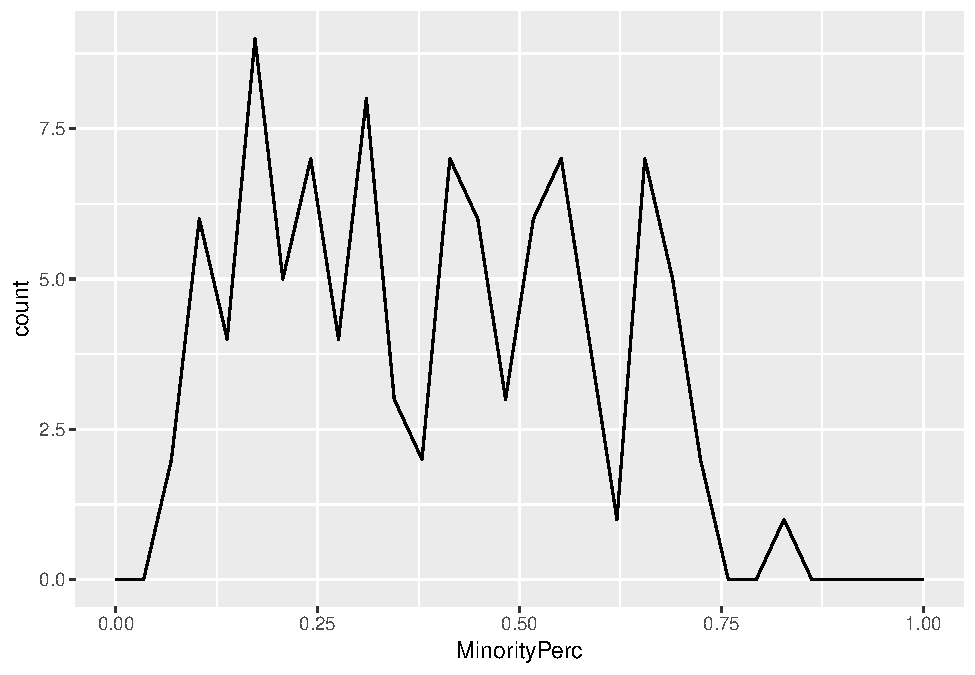
\includegraphics{Project_Template_files/figure-latex/exploratory graphs-1.pdf}

\begin{Shaded}
\begin{Highlighting}[]
\KeywordTok{qqnorm}\NormalTok{(Race_Processed}\OperatorTok{$}\NormalTok{MinorityPerc); }\KeywordTok{qqline}\NormalTok{(Race_Processed}\OperatorTok{$}\NormalTok{MinorityPerc)}
\end{Highlighting}
\end{Shaded}

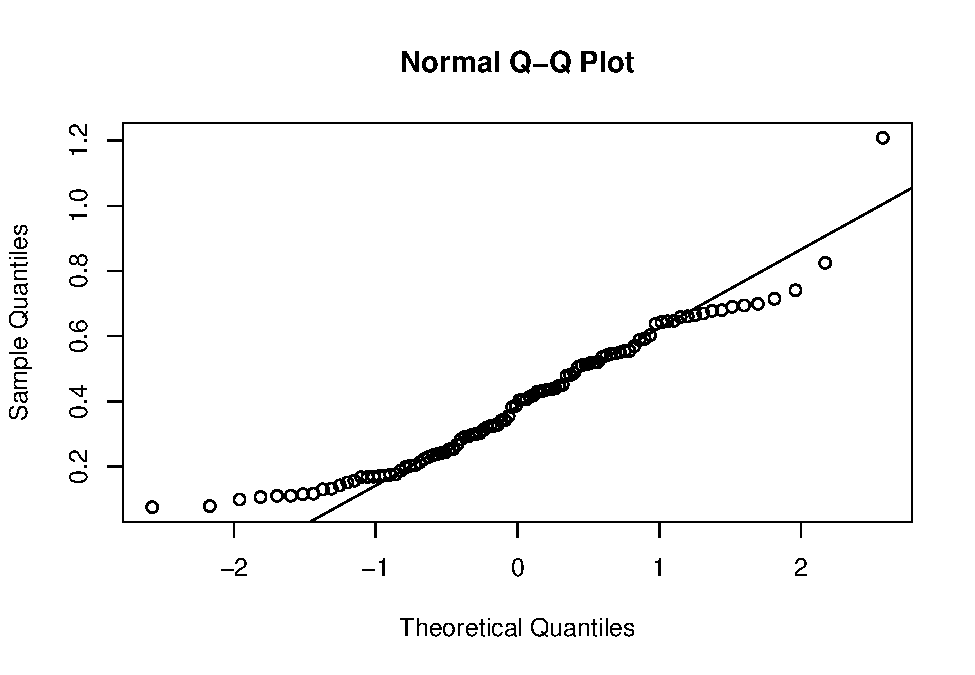
\includegraphics{Project_Template_files/figure-latex/exploratory graphs-2.pdf}

\begin{Shaded}
\begin{Highlighting}[]
\KeywordTok{ggplot}\NormalTok{(Poverty_NC, }\KeywordTok{aes}\NormalTok{(}\DataTypeTok{x =}\NormalTok{ Poverty_Percent_allages)) }\OperatorTok{+}
\StringTok{  }\KeywordTok{geom_freqpoly}\NormalTok{()}
\end{Highlighting}
\end{Shaded}

\begin{verbatim}
## `stat_bin()` using `bins = 30`. Pick better value with `binwidth`.
\end{verbatim}

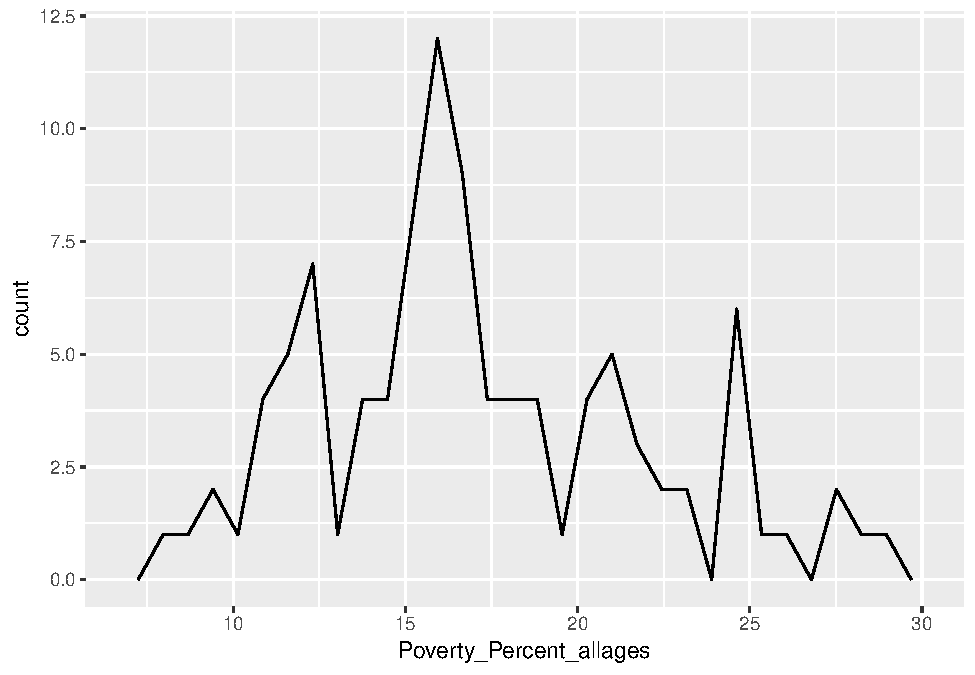
\includegraphics{Project_Template_files/figure-latex/exploratory graphs-3.pdf}

\begin{Shaded}
\begin{Highlighting}[]
\KeywordTok{qqnorm}\NormalTok{(Poverty_NC}\OperatorTok{$}\NormalTok{Poverty_Percent_allages); }\KeywordTok{qqline}\NormalTok{(Poverty_NC}\OperatorTok{$}\NormalTok{Poverty_Percent_allages)}
\end{Highlighting}
\end{Shaded}

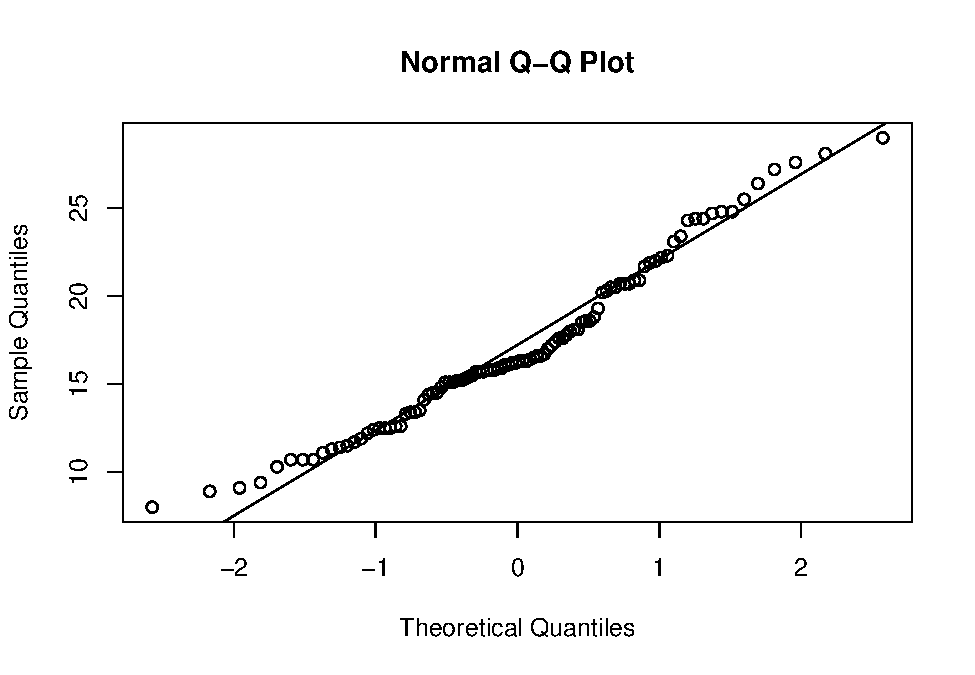
\includegraphics{Project_Template_files/figure-latex/exploratory graphs-4.pdf}

\section{Read in Counties shapefile into an sf dataframe, filtering for
just NC
counties}\label{read-in-counties-shapefile-into-an-sf-dataframe-filtering-for-just-nc-counties}

\begin{Shaded}
\begin{Highlighting}[]
\CommentTok{#Read in Counties shapefile into an sf dataframe, filtering for just NC counties}

\NormalTok{NC_Counties_shp <-}\StringTok{ }\KeywordTok{st_read}\NormalTok{(}\DataTypeTok{dsn =} \StringTok{"./Data/Spatial/NC_Counties.shp"}\NormalTok{) }\CommentTok{#Geospatial data for NC Counties}
\end{Highlighting}
\end{Shaded}

\begin{verbatim}
## Reading layer `NC_Counties' from data source `/Users/Tristen/OneDrive - Duke University/Spring 2019/Data Analytics/EJ_Project/Data/Spatial/NC_Counties.shp' using driver `ESRI Shapefile'
## Simple feature collection with 100 features and 9 fields
## geometry type:  POLYGON
## dimension:      XY
## bbox:           xmin: -84.32162 ymin: 33.83437 xmax: -75.45998 ymax: 36.58841
## epsg (SRID):    4326
## proj4string:    +proj=longlat +datum=WGS84 +no_defs
\end{verbatim}

\begin{Shaded}
\begin{Highlighting}[]
\NormalTok{Landfills_shp <-}\StringTok{ }\KeywordTok{st_read}\NormalTok{(}\DataTypeTok{dsn =} \StringTok{"./Data/Spatial/ActivePermittedLandiflls.shp"}\NormalTok{) }\CommentTok{#Active Landfills}
\end{Highlighting}
\end{Shaded}

\begin{verbatim}
## Reading layer `ActivePermittedLandiflls' from data source `/Users/Tristen/OneDrive - Duke University/Spring 2019/Data Analytics/EJ_Project/Data/Spatial/ActivePermittedLandiflls.shp' using driver `ESRI Shapefile'
## Simple feature collection with 177 features and 9 fields
## geometry type:  POINT
## dimension:      XY
## bbox:           xmin: -1.797693e+308 ymin: -1.797693e+308 xmax: -75.49015 ymax: 36.5332
## epsg (SRID):    4326
## proj4string:    +proj=longlat +datum=WGS84 +no_defs
\end{verbatim}

\begin{Shaded}
\begin{Highlighting}[]
\NormalTok{IH_shp <-}\StringTok{ }\KeywordTok{st_read}\NormalTok{(}\DataTypeTok{dsn =} \StringTok{"./Data/Spatial/IH_Sites.shp"}\NormalTok{) }\CommentTok{#Hazardous substance spill and disposal sites }
\end{Highlighting}
\end{Shaded}

\begin{verbatim}
## Reading layer `IH_Sites' from data source `/Users/Tristen/OneDrive - Duke University/Spring 2019/Data Analytics/EJ_Project/Data/Spatial/IH_Sites.shp' using driver `ESRI Shapefile'
## Simple feature collection with 1917 features and 13 fields
## geometry type:  POINT
## dimension:      XY
## bbox:           xmin: -83.96576 ymin: 33.9127 xmax: -75.52278 ymax: 36.54823
## epsg (SRID):    4326
## proj4string:    +proj=longlat +datum=WGS84 +no_defs
\end{verbatim}

\begin{Shaded}
\begin{Highlighting}[]
\NormalTok{FRB_shp <-}\StringTok{ }\KeywordTok{st_read}\NormalTok{(}\DataTypeTok{dsn =} \StringTok{"./Data/Spatial/FRB_Sites.shp"}\NormalTok{) }\CommentTok{#Superfund}
\end{Highlighting}
\end{Shaded}

\begin{verbatim}
## Reading layer `FRB_Sites' from data source `/Users/Tristen/OneDrive - Duke University/Spring 2019/Data Analytics/EJ_Project/Data/Spatial/FRB_Sites.shp' using driver `ESRI Shapefile'
## Simple feature collection with 70 features and 24 fields
## geometry type:  POINT
## dimension:      XY
## bbox:           xmin: -9246629 ymin: 4057672 xmax: -8407034 ymax: 4358145
## epsg (SRID):    3857
## proj4string:    +proj=merc +a=6378137 +b=6378137 +lat_ts=0.0 +lon_0=0.0 +x_0=0.0 +y_0=0 +k=1.0 +units=m +nadgrids=@null +wktext +no_defs
\end{verbatim}

\begin{Shaded}
\begin{Highlighting}[]
\NormalTok{BF_shp <-}\StringTok{ }\KeywordTok{st_read}\NormalTok{(}\DataTypeTok{dsn =} \StringTok{"./Data/Spatial/BF_Sites.shp"}\NormalTok{) }\CommentTok{#Brownfields}
\end{Highlighting}
\end{Shaded}

\begin{verbatim}
## Reading layer `BF_Sites' from data source `/Users/Tristen/OneDrive - Duke University/Spring 2019/Data Analytics/EJ_Project/Data/Spatial/BF_Sites.shp' using driver `ESRI Shapefile'
## Simple feature collection with 398 features and 9 fields
## geometry type:  POINT
## dimension:      XY
## bbox:           xmin: 693972.8 ymin: 174551.3 xmax: 2827425 ymax: 1024565
## epsg (SRID):    NA
## proj4string:    +proj=lcc +lat_1=34.33333333333334 +lat_2=36.16666666666666 +lat_0=33.75 +lon_0=-79 +x_0=609601.2199999997 +y_0=0 +datum=NAD83 +units=us-ft +no_defs
\end{verbatim}

\begin{Shaded}
\begin{Highlighting}[]
\NormalTok{RUST_shp <-}\StringTok{ }\KeywordTok{st_read}\NormalTok{(}\DataTypeTok{dsn =} \StringTok{"./Data/Spatial/RUST.shp"}\NormalTok{) }\CommentTok{#Underground Storage Tanks}
\end{Highlighting}
\end{Shaded}

\begin{verbatim}
## Reading layer `RUST' from data source `/Users/Tristen/OneDrive - Duke University/Spring 2019/Data Analytics/EJ_Project/Data/Spatial/RUST.shp' using driver `ESRI Shapefile'
## Simple feature collection with 30212 features and 28 fields
## geometry type:  POINT
## dimension:      XY
## bbox:           xmin: -84.31466 ymin: 33.87549 xmax: -75.46581 ymax: 36.567
## epsg (SRID):    4326
## proj4string:    +proj=longlat +datum=WGS84 +no_defs
\end{verbatim}

\begin{Shaded}
\begin{Highlighting}[]
\NormalTok{HW_shp <-}\StringTok{ }\KeywordTok{st_read}\NormalTok{(}\DataTypeTok{dsn =} \StringTok{"./Data/Spatial/HW_Sites.shp"}\NormalTok{) }\CommentTok{#Hazardous Waste Resource Conservation and Recovery Act}
\end{Highlighting}
\end{Shaded}

\begin{verbatim}
## Reading layer `HW_Sites' from data source `/Users/Tristen/OneDrive - Duke University/Spring 2019/Data Analytics/EJ_Project/Data/Spatial/HW_Sites.shp' using driver `ESRI Shapefile'
## Simple feature collection with 2577 features and 21 fields
## geometry type:  POINT
## dimension:      XY
## bbox:           xmin: -84.02775 ymin: 33.89647 xmax: -75.60355 ymax: 36.53089
## epsg (SRID):    4326
## proj4string:    +proj=longlat +datum=WGS84 +no_defs
\end{verbatim}

\begin{Shaded}
\begin{Highlighting}[]
\CommentTok{#Reveal the CRS of the counties features so they can be graphed with NC Counties shapefile}
\KeywordTok{st_crs}\NormalTok{(NC_Counties_shp)}
\end{Highlighting}
\end{Shaded}

\begin{verbatim}
## Coordinate Reference System:
##   EPSG: 4326 
##   proj4string: "+proj=longlat +datum=WGS84 +no_defs"
\end{verbatim}

\begin{Shaded}
\begin{Highlighting}[]
\KeywordTok{st_crs}\NormalTok{(Landfills_shp)}
\end{Highlighting}
\end{Shaded}

\begin{verbatim}
## Coordinate Reference System:
##   EPSG: 4326 
##   proj4string: "+proj=longlat +datum=WGS84 +no_defs"
\end{verbatim}

\begin{Shaded}
\begin{Highlighting}[]
\KeywordTok{st_crs}\NormalTok{(IH_shp)}
\end{Highlighting}
\end{Shaded}

\begin{verbatim}
## Coordinate Reference System:
##   EPSG: 4326 
##   proj4string: "+proj=longlat +datum=WGS84 +no_defs"
\end{verbatim}

\begin{Shaded}
\begin{Highlighting}[]
\KeywordTok{st_crs}\NormalTok{(FRB_shp)}
\end{Highlighting}
\end{Shaded}

\begin{verbatim}
## Coordinate Reference System:
##   EPSG: 3857 
##   proj4string: "+proj=merc +a=6378137 +b=6378137 +lat_ts=0.0 +lon_0=0.0 +x_0=0.0 +y_0=0 +k=1.0 +units=m +nadgrids=@null +wktext +no_defs"
\end{verbatim}

\begin{Shaded}
\begin{Highlighting}[]
\KeywordTok{st_crs}\NormalTok{(BF_shp)}
\end{Highlighting}
\end{Shaded}

\begin{verbatim}
## Coordinate Reference System:
##   No EPSG code
##   proj4string: "+proj=lcc +lat_1=34.33333333333334 +lat_2=36.16666666666666 +lat_0=33.75 +lon_0=-79 +x_0=609601.2199999997 +y_0=0 +datum=NAD83 +units=us-ft +no_defs"
\end{verbatim}

\begin{Shaded}
\begin{Highlighting}[]
\KeywordTok{st_crs}\NormalTok{(RUST_shp)}
\end{Highlighting}
\end{Shaded}

\begin{verbatim}
## Coordinate Reference System:
##   EPSG: 4326 
##   proj4string: "+proj=longlat +datum=WGS84 +no_defs"
\end{verbatim}

\begin{Shaded}
\begin{Highlighting}[]
\KeywordTok{st_crs}\NormalTok{(HW_shp)}
\end{Highlighting}
\end{Shaded}

\begin{verbatim}
## Coordinate Reference System:
##   EPSG: 4326 
##   proj4string: "+proj=longlat +datum=WGS84 +no_defs"
\end{verbatim}

\begin{Shaded}
\begin{Highlighting}[]
\CommentTok{#There is one row with an incorecct location; This site will be omitted in order to proceed with mapping data}
\NormalTok{Landfills_shp_mod <-}\StringTok{ }\KeywordTok{subset}\NormalTok{(Landfills_shp, }\OperatorTok{!}\NormalTok{LocationID }\OperatorTok{==}\StringTok{ "P1252"}\NormalTok{)}

\CommentTok{#Filter RUST dataset for only high risk UST sites since this inforation is available and due to the large amount of sites}
\KeywordTok{levels}\NormalTok{(RUST_shp}\OperatorTok{$}\NormalTok{ConfRisk)}
\end{Highlighting}
\end{Shaded}

\begin{verbatim}
## [1] "H" "I" "l" "L" "U"
\end{verbatim}

\begin{Shaded}
\begin{Highlighting}[]
\NormalTok{highrisk_RUST <-}\StringTok{ }\NormalTok{RUST_shp }\OperatorTok
\StringTok{  }\KeywordTok{filter}\NormalTok{(ConfRisk }\OperatorTok{==}\StringTok{ "H"}\NormalTok{)}

\CommentTok{#Join poverty data to county geospatial data}
\NormalTok{county_poverty_join <-}\StringTok{ }\NormalTok{NC_Counties_shp }\OperatorTok\StringTok{ }
\StringTok{  }\KeywordTok{left_join}\NormalTok{(}\DataTypeTok{y =}\NormalTok{ Poverty_NC,}\DataTypeTok{by =} \KeywordTok{c}\NormalTok{(}\StringTok{"CO_NAME"}\NormalTok{ =}\StringTok{  "Name"}\NormalTok{))}


\CommentTok{#Count the number of sites in each county; In some, the names of counties are not in all capital letters. In order to address future problems with joins, some were converted to all capital letters.}
\NormalTok{Sitecount_Landfill <-}\StringTok{ }\KeywordTok{count}\NormalTok{(Landfills_shp_mod, Landfills_shp_mod}\OperatorTok{$}\NormalTok{County)}

\KeywordTok{levels}\NormalTok{(IH_shp}\OperatorTok{$}\NormalTok{SITECOUNTY) <-}\StringTok{ }\KeywordTok{toupper}\NormalTok{(}\KeywordTok{levels}\NormalTok{(IH_shp}\OperatorTok{$}\NormalTok{SITECOUNTY)) }\CommentTok{#all caps}
\NormalTok{Sitecount_IH <-}\StringTok{ }\KeywordTok{count}\NormalTok{(IH_shp, IH_shp}\OperatorTok{$}\NormalTok{SITECOUNTY) }

\NormalTok{Sitecount_FRB <-}\StringTok{ }\KeywordTok{count}\NormalTok{(FRB_shp, FRB_shp}\OperatorTok{$}\NormalTok{SITE_COUNT) }

\KeywordTok{levels}\NormalTok{(BF_shp}\OperatorTok{$}\NormalTok{BF_County) <-}\StringTok{ }\KeywordTok{toupper}\NormalTok{(}\KeywordTok{levels}\NormalTok{(BF_shp}\OperatorTok{$}\NormalTok{BF_County))}
\NormalTok{Sitecount_BF <-}\StringTok{ }\KeywordTok{count}\NormalTok{(BF_shp, BF_shp}\OperatorTok{$}\NormalTok{BF_County)}

\KeywordTok{levels}\NormalTok{(highrisk_RUST}\OperatorTok{$}\NormalTok{County) <-}\StringTok{ }\KeywordTok{toupper}\NormalTok{(}\KeywordTok{levels}\NormalTok{(highrisk_RUST}\OperatorTok{$}\NormalTok{County))}
\NormalTok{Sitecount_RUST <-}\StringTok{ }\KeywordTok{count}\NormalTok{(highrisk_RUST, highrisk_RUST}\OperatorTok{$}\NormalTok{County)}

\NormalTok{Sitecount_HW <-}\StringTok{ }\KeywordTok{count}\NormalTok{(HW_shp, HW_shp}\OperatorTok{$}\NormalTok{LOC_COUNTY)}


\CommentTok{#Join count dataframes with race info. Needed to make county names in Race_Processed data set capitalized so left join would work. In one case, Race_Processed data needed to add a column with abbreviations in order to join to the RUST data set.}
\NormalTok{Sitecount_Landfill_join <-}\StringTok{ }\KeywordTok{left_join}\NormalTok{(Sitecount_Landfill, Race_Processed, }\DataTypeTok{by =} \KeywordTok{c}\NormalTok{(}\StringTok{"Landfills_shp_mod$County"}\NormalTok{ =}\StringTok{ "County"}\NormalTok{))}
\end{Highlighting}
\end{Shaded}

\begin{verbatim}
## Warning: Column `Landfills_shp_mod$County`/`County` joining factors with
## different levels, coercing to character vector
\end{verbatim}

\begin{Shaded}
\begin{Highlighting}[]
\KeywordTok{levels}\NormalTok{(Race_Processed}\OperatorTok{$}\NormalTok{County) <-}\StringTok{ }\KeywordTok{toupper}\NormalTok{(}\KeywordTok{levels}\NormalTok{(Race_Processed}\OperatorTok{$}\NormalTok{County))}
\NormalTok{Sitecount_IH_join <-}\StringTok{ }\KeywordTok{left_join}\NormalTok{(Sitecount_IH, Race_Processed, }\DataTypeTok{by =} \KeywordTok{c}\NormalTok{(}\StringTok{"IH_shp$SITECOUNTY"}\NormalTok{ =}\StringTok{ "County"}\NormalTok{))}
\end{Highlighting}
\end{Shaded}

\begin{verbatim}
## Warning: Column `IH_shp$SITECOUNTY`/`County` joining factors with different
## levels, coercing to character vector
\end{verbatim}

\begin{Shaded}
\begin{Highlighting}[]
\NormalTok{Sitecount_FRB_join <-}\StringTok{ }\KeywordTok{left_join}\NormalTok{(Sitecount_FRB, Race_Processed, }
  \DataTypeTok{by =} \KeywordTok{c}\NormalTok{(}\StringTok{"FRB_shp$SITE_COUNT"}\NormalTok{ =}\StringTok{ "County"}\NormalTok{))}
\end{Highlighting}
\end{Shaded}

\begin{verbatim}
## Warning: Column `FRB_shp$SITE_COUNT`/`County` joining factors with
## different levels, coercing to character vector
\end{verbatim}

\begin{Shaded}
\begin{Highlighting}[]
\NormalTok{Sitecount_BF_join <-}\StringTok{ }\KeywordTok{left_join}\NormalTok{(Sitecount_BF, Race_Processed, }\DataTypeTok{by =} \KeywordTok{c}\NormalTok{(}\StringTok{"BF_shp$BF_County"}\NormalTok{ =}\StringTok{ "County"}\NormalTok{))}
\end{Highlighting}
\end{Shaded}

\begin{verbatim}
## Warning: Column `BF_shp$BF_County`/`County` joining factors with different
## levels, coercing to character vector
\end{verbatim}

\begin{Shaded}
\begin{Highlighting}[]
\NormalTok{Race_Processed_abv <-}\StringTok{ }\KeywordTok{transform}\NormalTok{(Race_Processed, }\DataTypeTok{ABV =} \KeywordTok{str_sub}\NormalTok{(Race_Processed}\OperatorTok{$}\NormalTok{County, }\DecValTok{1}\NormalTok{, }\DecValTok{5}\NormalTok{))}

\NormalTok{Sitecount_RUST_join <-}\StringTok{ }\KeywordTok{left_join}\NormalTok{(Sitecount_RUST, Race_Processed_abv, }\DataTypeTok{by =} \KeywordTok{c}\NormalTok{(}\StringTok{"highrisk_RUST$County"}\NormalTok{ =}\StringTok{ "ABV"}\NormalTok{))}
\end{Highlighting}
\end{Shaded}

\begin{verbatim}
## Warning: Column `highrisk_RUST$County`/`ABV` joining factors with different
## levels, coercing to character vector
\end{verbatim}

\begin{Shaded}
\begin{Highlighting}[]
\NormalTok{Sitecount_HW_join <-}\StringTok{ }\KeywordTok{left_join}\NormalTok{(Sitecount_HW, Race_Processed, }\DataTypeTok{by =} \KeywordTok{c}\NormalTok{(}\StringTok{"HW_shp$LOC_COUNTY"}\NormalTok{ =}\StringTok{ "County"}\NormalTok{))}
\end{Highlighting}
\end{Shaded}

\begin{verbatim}
## Warning: Column `HW_shp$LOC_COUNTY`/`County` joining factors with different
## levels, coercing to character vector
\end{verbatim}

\newpage

\section{Analysis}\label{analysis}

\begin{Shaded}
\begin{Highlighting}[]
\CommentTok{#Creating maps from basic data with counties}
\KeywordTok{ggplot}\NormalTok{() }\OperatorTok{+}\StringTok{ }
\StringTok{  }\KeywordTok{geom_sf}\NormalTok{(}\DataTypeTok{data =}\NormalTok{ county_poverty_join, }\KeywordTok{aes}\NormalTok{(}\DataTypeTok{fill=}\NormalTok{county_poverty_join}\OperatorTok{$}\NormalTok{Poverty_Percent_allages)) }\OperatorTok{+}
\StringTok{  }\KeywordTok{scale_fill_viridis}\NormalTok{(}\DataTypeTok{direction =} \OperatorTok{-}\DecValTok{1}\NormalTok{) }\OperatorTok{+}
\StringTok{  }\KeywordTok{geom_sf}\NormalTok{(}\DataTypeTok{data =}\NormalTok{ Landfills_shp_mod, }\DataTypeTok{alpha =} \FloatTok{0.6}\NormalTok{) }\OperatorTok{+}
\StringTok{ }\KeywordTok{labs}\NormalTok{(}\DataTypeTok{fill =} \StringTok{"% in Poverty"}\NormalTok{) }\OperatorTok{+}
\StringTok{  }\KeywordTok{ggtitle}\NormalTok{(}\StringTok{"Landfill Sites in North Carolina"}\NormalTok{)}
\end{Highlighting}
\end{Shaded}

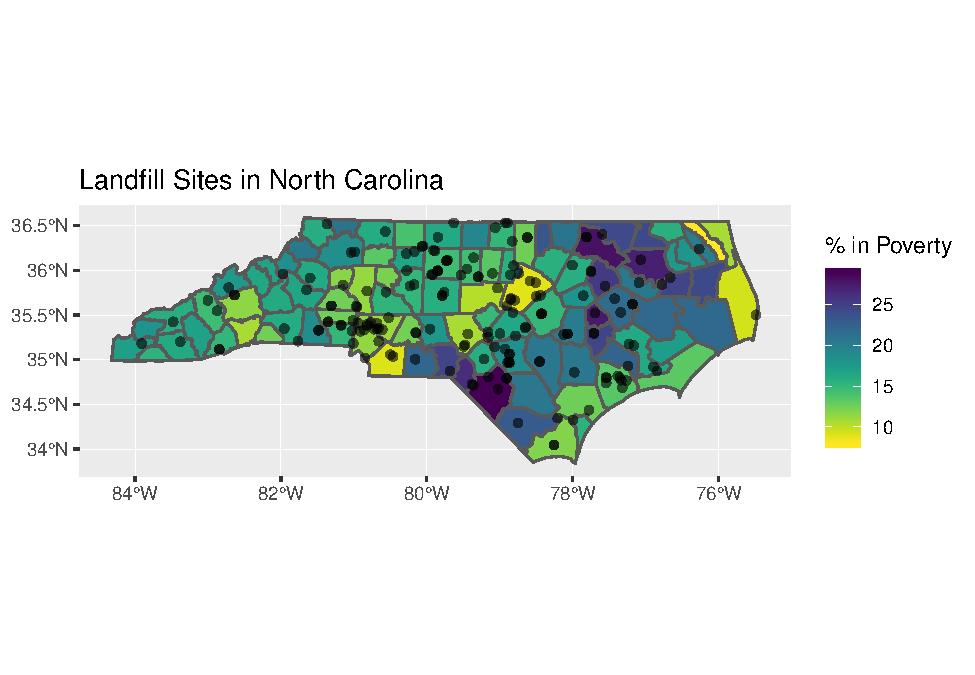
\includegraphics{Project_Template_files/figure-latex/final visualizations-1.pdf}

\begin{Shaded}
\begin{Highlighting}[]
\KeywordTok{ggplot}\NormalTok{() }\OperatorTok{+}\StringTok{ }
\StringTok{  }\KeywordTok{geom_sf}\NormalTok{(}\DataTypeTok{data =}\NormalTok{ county_poverty_join, }\KeywordTok{aes}\NormalTok{(}\DataTypeTok{fill=}\NormalTok{county_poverty_join}\OperatorTok{$}\NormalTok{Poverty_Percent_allages)) }\OperatorTok{+}
\StringTok{  }\KeywordTok{scale_fill_viridis}\NormalTok{(}\DataTypeTok{direction =} \OperatorTok{-}\DecValTok{1}\NormalTok{) }\OperatorTok{+}
\StringTok{  }\KeywordTok{geom_sf}\NormalTok{(}\DataTypeTok{data =}\NormalTok{ IH_shp, }\DataTypeTok{alpha =} \FloatTok{0.3}\NormalTok{, }\DataTypeTok{color =} \StringTok{"black"}\NormalTok{) }\OperatorTok{+}
\StringTok{ }\KeywordTok{labs}\NormalTok{(}\DataTypeTok{fill =} \StringTok{"% in Poverty"}\NormalTok{) }\OperatorTok{+}
\StringTok{  }\KeywordTok{ggtitle}\NormalTok{(}\StringTok{"IH Sites in North Carolina"}\NormalTok{)}
\end{Highlighting}
\end{Shaded}

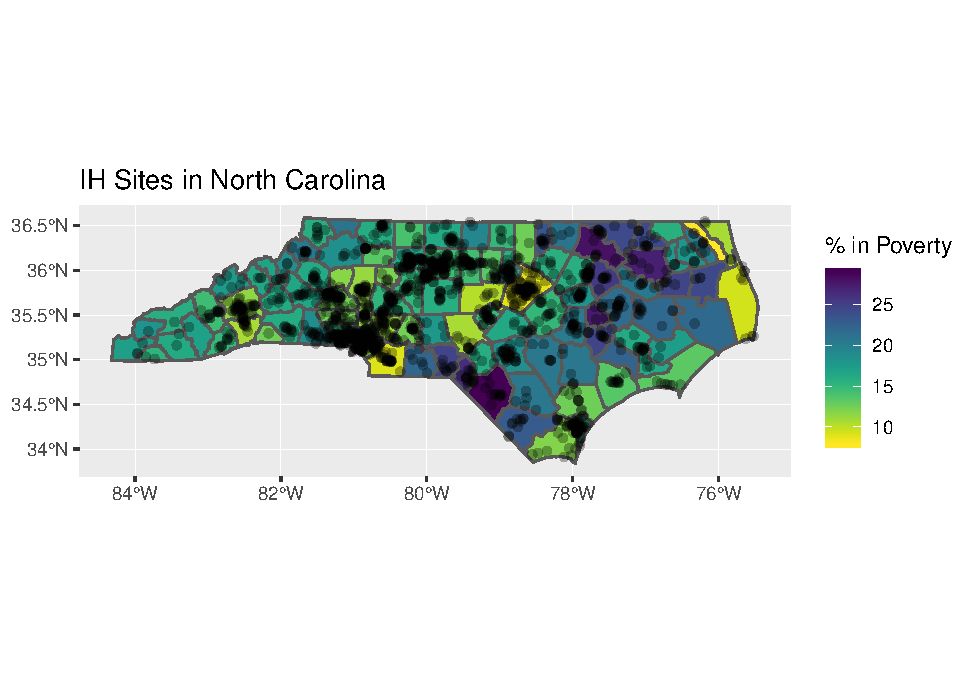
\includegraphics{Project_Template_files/figure-latex/final visualizations-2.pdf}

\begin{Shaded}
\begin{Highlighting}[]
\KeywordTok{ggplot}\NormalTok{() }\OperatorTok{+}\StringTok{ }
\StringTok{  }\KeywordTok{geom_sf}\NormalTok{(}\DataTypeTok{data =}\NormalTok{ county_poverty_join, }\KeywordTok{aes}\NormalTok{(}\DataTypeTok{fill=}\NormalTok{county_poverty_join}\OperatorTok{$}\NormalTok{Poverty_Percent_allages)) }\OperatorTok{+}
\StringTok{  }\KeywordTok{scale_fill_viridis}\NormalTok{(}\DataTypeTok{direction =} \OperatorTok{-}\DecValTok{1}\NormalTok{) }\OperatorTok{+}
\StringTok{  }\KeywordTok{geom_sf}\NormalTok{(}\DataTypeTok{data =}\NormalTok{ FRB_shp, }\DataTypeTok{alpha =} \FloatTok{0.6}\NormalTok{, }\DataTypeTok{color =} \StringTok{"black"}\NormalTok{) }\OperatorTok{+}
\StringTok{ }\KeywordTok{labs}\NormalTok{(}\DataTypeTok{fill =} \StringTok{"% in Poverty"}\NormalTok{) }\OperatorTok{+}
\StringTok{  }\KeywordTok{ggtitle}\NormalTok{(}\StringTok{"Superfund Sites in North Carolina"}\NormalTok{)}
\end{Highlighting}
\end{Shaded}

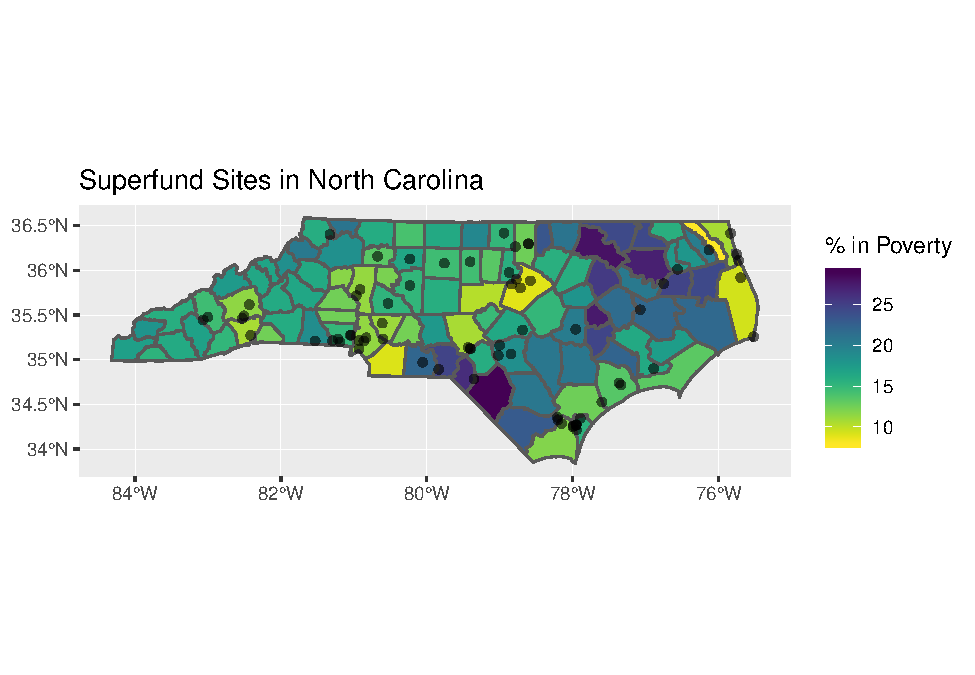
\includegraphics{Project_Template_files/figure-latex/final visualizations-3.pdf}

\begin{Shaded}
\begin{Highlighting}[]
\KeywordTok{ggplot}\NormalTok{() }\OperatorTok{+}\StringTok{ }
\StringTok{  }\KeywordTok{geom_sf}\NormalTok{(}\DataTypeTok{data =}\NormalTok{ county_poverty_join, }\KeywordTok{aes}\NormalTok{(}\DataTypeTok{fill=}\NormalTok{county_poverty_join}\OperatorTok{$}\NormalTok{Poverty_Percent_allages)) }\OperatorTok{+}
\StringTok{  }\KeywordTok{scale_fill_viridis}\NormalTok{(}\DataTypeTok{direction =} \OperatorTok{-}\DecValTok{1}\NormalTok{) }\OperatorTok{+}
\StringTok{  }\KeywordTok{geom_sf}\NormalTok{(}\DataTypeTok{data =}\NormalTok{ BF_shp, }\DataTypeTok{alpha =} \FloatTok{0.4}\NormalTok{) }\OperatorTok{+}
\StringTok{ }\KeywordTok{labs}\NormalTok{(}\DataTypeTok{fill =} \StringTok{"% in Poverty"}\NormalTok{) }\OperatorTok{+}
\StringTok{  }\KeywordTok{ggtitle}\NormalTok{(}\StringTok{"Brownfield Sites in North Carolina"}\NormalTok{)}
\end{Highlighting}
\end{Shaded}

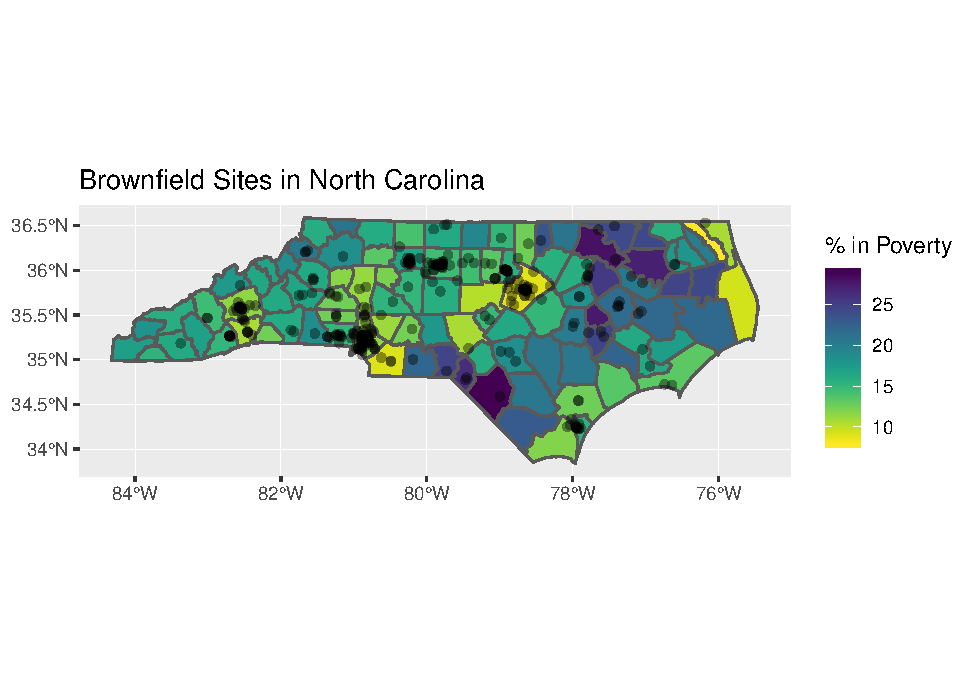
\includegraphics{Project_Template_files/figure-latex/final visualizations-4.pdf}

\begin{Shaded}
\begin{Highlighting}[]
\KeywordTok{ggplot}\NormalTok{() }\OperatorTok{+}\StringTok{ }
\StringTok{  }\KeywordTok{geom_sf}\NormalTok{(}\DataTypeTok{data =}\NormalTok{ county_poverty_join, }\KeywordTok{aes}\NormalTok{(}\DataTypeTok{fill=}\NormalTok{county_poverty_join}\OperatorTok{$}\NormalTok{Poverty_Percent_allages)) }\OperatorTok{+}
\StringTok{  }\KeywordTok{scale_fill_viridis}\NormalTok{(}\DataTypeTok{direction =} \OperatorTok{-}\DecValTok{1}\NormalTok{) }\OperatorTok{+}
\StringTok{  }\KeywordTok{geom_sf}\NormalTok{(}\DataTypeTok{data =}\NormalTok{ highrisk_RUST, }\DataTypeTok{alpha =} \FloatTok{0.3}\NormalTok{, }\DataTypeTok{color =} \StringTok{"black"}\NormalTok{) }\OperatorTok{+}
\StringTok{ }\KeywordTok{labs}\NormalTok{(}\DataTypeTok{fill =} \StringTok{"% in Poverty"}\NormalTok{) }\OperatorTok{+}
\StringTok{  }\KeywordTok{ggtitle}\NormalTok{(}\StringTok{"RUST Sites in North Carolina"}\NormalTok{)}
\end{Highlighting}
\end{Shaded}

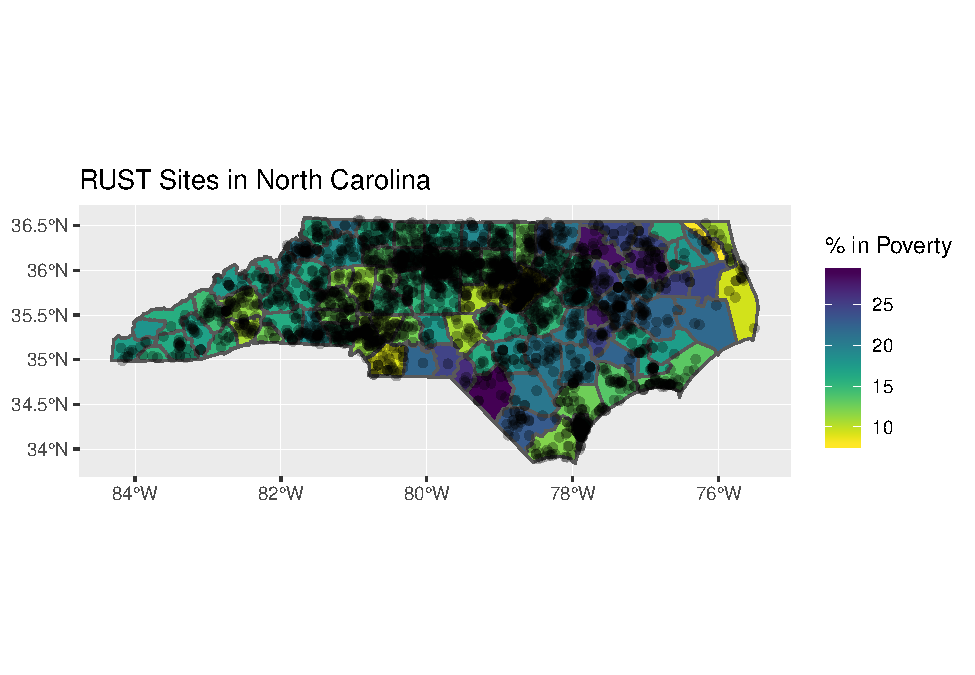
\includegraphics{Project_Template_files/figure-latex/final visualizations-5.pdf}

\begin{Shaded}
\begin{Highlighting}[]
\KeywordTok{ggplot}\NormalTok{() }\OperatorTok{+}\StringTok{ }
\StringTok{  }\KeywordTok{geom_sf}\NormalTok{(}\DataTypeTok{data =}\NormalTok{ county_poverty_join, }\KeywordTok{aes}\NormalTok{(}\DataTypeTok{fill=}\NormalTok{county_poverty_join}\OperatorTok{$}\NormalTok{Poverty_Percent_allages)) }\OperatorTok{+}
\StringTok{  }\KeywordTok{scale_fill_viridis}\NormalTok{(}\DataTypeTok{direction =} \OperatorTok{-}\DecValTok{1}\NormalTok{) }\OperatorTok{+}
\StringTok{  }\KeywordTok{geom_sf}\NormalTok{(}\DataTypeTok{data =}\NormalTok{ HW_shp, }\DataTypeTok{alpha =} \FloatTok{0.3}\NormalTok{, }\DataTypeTok{color =} \StringTok{"black"}\NormalTok{) }\OperatorTok{+}
\StringTok{ }\KeywordTok{labs}\NormalTok{(}\DataTypeTok{fill =} \StringTok{"% in Poverty"}\NormalTok{) }\OperatorTok{+}
\StringTok{  }\KeywordTok{ggtitle}\NormalTok{(}\StringTok{"Hazardous Waste Sites in North Carolina"}\NormalTok{)}
\end{Highlighting}
\end{Shaded}

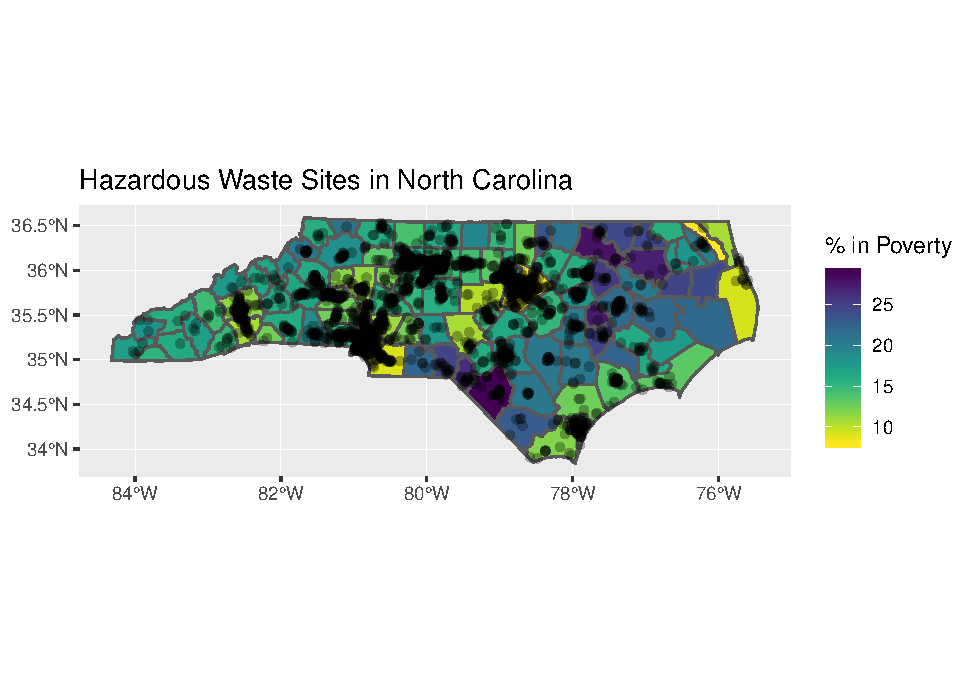
\includegraphics{Project_Template_files/figure-latex/final visualizations-6.pdf}

\begin{Shaded}
\begin{Highlighting}[]
\CommentTok{#Graph count data with race percent data}
\NormalTok{Landfill_plot <-}\StringTok{ }
\StringTok{  }\KeywordTok{ggplot}\NormalTok{(Sitecount_Landfill_join, }\KeywordTok{aes}\NormalTok{(}\DataTypeTok{x=}\NormalTok{n , }\DataTypeTok{y=}\NormalTok{MinorityPerc }\OperatorTok{*}\StringTok{ }\DecValTok{100}\NormalTok{)) }\OperatorTok{+}
\StringTok{  }\KeywordTok{scale_y_continuous}\NormalTok{(}\DataTypeTok{limits=}\KeywordTok{c}\NormalTok{(}\DecValTok{0}\NormalTok{, }\DecValTok{100}\NormalTok{)) }\OperatorTok{+}
\StringTok{  }\KeywordTok{geom_point}\NormalTok{(}\DataTypeTok{alpha=}\FloatTok{0.7}\NormalTok{, }\DataTypeTok{color=}\StringTok{"blue"}\NormalTok{) }\OperatorTok{+}
\StringTok{  }\KeywordTok{labs}\NormalTok{(}\DataTypeTok{x=}\StringTok{"Site Count"}\NormalTok{, }\DataTypeTok{y=}\StringTok{"Racial Minority Percent"}\NormalTok{)}

\NormalTok{IH_plot <-}\StringTok{ }
\StringTok{  }\KeywordTok{ggplot}\NormalTok{(Sitecount_IH_join, }\KeywordTok{aes}\NormalTok{(}\DataTypeTok{x=}\NormalTok{n , }\DataTypeTok{y=}\NormalTok{MinorityPerc }\OperatorTok{*}\StringTok{ }\DecValTok{100}\NormalTok{)) }\OperatorTok{+}
\StringTok{  }\KeywordTok{scale_y_continuous}\NormalTok{(}\DataTypeTok{limits=}\KeywordTok{c}\NormalTok{(}\DecValTok{0}\NormalTok{, }\DecValTok{100}\NormalTok{)) }\OperatorTok{+}
\StringTok{  }\KeywordTok{geom_point}\NormalTok{(}\DataTypeTok{alpha=}\FloatTok{0.7}\NormalTok{, }\DataTypeTok{color=}\StringTok{"blue"}\NormalTok{) }\OperatorTok{+}
\StringTok{  }\KeywordTok{labs}\NormalTok{(}\DataTypeTok{x=}\StringTok{"Site Count"}\NormalTok{, }\DataTypeTok{y=}\StringTok{"Racial Minority Percent"}\NormalTok{)}

\NormalTok{FRB_plot <-}\StringTok{ }
\StringTok{  }\KeywordTok{ggplot}\NormalTok{(Sitecount_FRB_join, }\KeywordTok{aes}\NormalTok{(}\DataTypeTok{x=}\NormalTok{n , }\DataTypeTok{y=}\NormalTok{MinorityPerc }\OperatorTok{*}\StringTok{ }\DecValTok{100}\NormalTok{)) }\OperatorTok{+}
\StringTok{  }\KeywordTok{scale_y_continuous}\NormalTok{(}\DataTypeTok{limits=}\KeywordTok{c}\NormalTok{(}\DecValTok{0}\NormalTok{, }\DecValTok{100}\NormalTok{)) }\OperatorTok{+}
\StringTok{  }\KeywordTok{geom_point}\NormalTok{(}\DataTypeTok{alpha=}\FloatTok{0.7}\NormalTok{) }\OperatorTok{+}
\StringTok{  }\KeywordTok{labs}\NormalTok{(}\DataTypeTok{x=}\StringTok{"Site Count"}\NormalTok{, }\DataTypeTok{y=}\StringTok{"Racial Minority Percent"}\NormalTok{)}
\NormalTok{FRB_plot}
\end{Highlighting}
\end{Shaded}

\begin{verbatim}
## Warning: Removed 4 rows containing missing values (geom_point).
\end{verbatim}

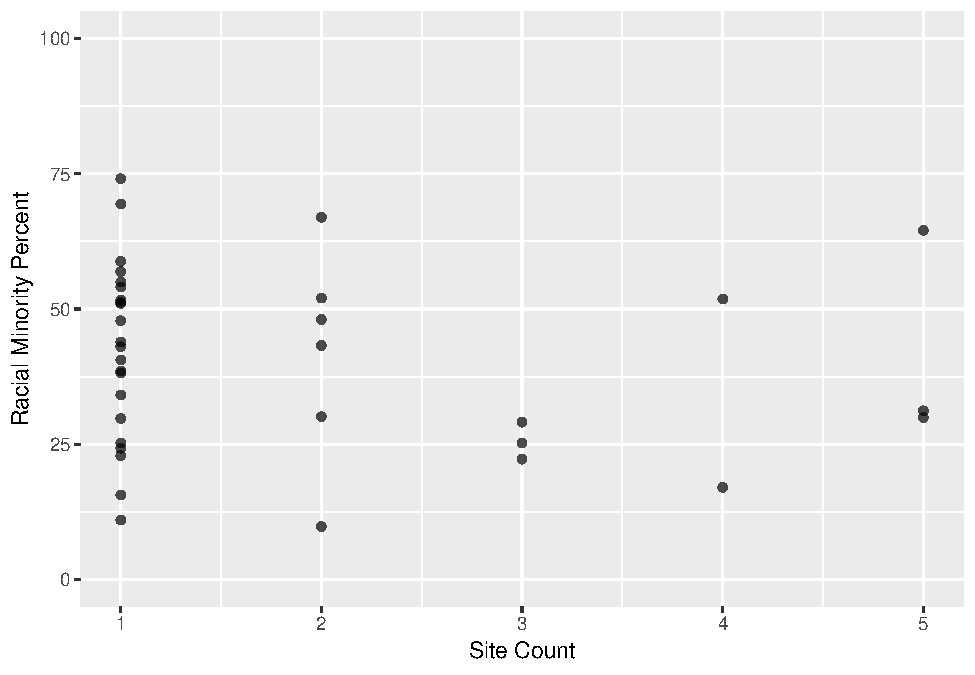
\includegraphics{Project_Template_files/figure-latex/final visualizations-7.pdf}

\begin{Shaded}
\begin{Highlighting}[]
\NormalTok{BF_plot <-}\StringTok{ }
\StringTok{  }\KeywordTok{ggplot}\NormalTok{(Sitecount_BF_join, }\KeywordTok{aes}\NormalTok{(}\DataTypeTok{x=}\NormalTok{n , }\DataTypeTok{y=}\NormalTok{MinorityPerc }\OperatorTok{*}\StringTok{ }\DecValTok{100}\NormalTok{)) }\OperatorTok{+}
\StringTok{  }\KeywordTok{scale_y_continuous}\NormalTok{(}\DataTypeTok{limits=}\KeywordTok{c}\NormalTok{(}\DecValTok{0}\NormalTok{, }\DecValTok{100}\NormalTok{)) }\OperatorTok{+}
\StringTok{  }\KeywordTok{geom_point}\NormalTok{(}\DataTypeTok{alpha=}\FloatTok{0.7}\NormalTok{, }\DataTypeTok{color=}\StringTok{"blue"}\NormalTok{) }\OperatorTok{+}
\StringTok{  }\KeywordTok{labs}\NormalTok{(}\DataTypeTok{x=}\StringTok{"Site Count"}\NormalTok{, }\DataTypeTok{y=}\StringTok{"Racial Minority Percent"}\NormalTok{)}

\NormalTok{RUST_plot <-}\StringTok{ }
\StringTok{  }\KeywordTok{ggplot}\NormalTok{(Sitecount_RUST_join, }\KeywordTok{aes}\NormalTok{(}\DataTypeTok{x=}\NormalTok{n , }\DataTypeTok{y=}\NormalTok{MinorityPerc }\OperatorTok{*}\StringTok{ }\DecValTok{100}\NormalTok{)) }\OperatorTok{+}
\StringTok{  }\KeywordTok{scale_y_continuous}\NormalTok{(}\DataTypeTok{limits=}\KeywordTok{c}\NormalTok{(}\DecValTok{0}\NormalTok{, }\DecValTok{100}\NormalTok{)) }\OperatorTok{+}
\StringTok{  }\KeywordTok{geom_point}\NormalTok{(}\DataTypeTok{alpha=}\FloatTok{0.7}\NormalTok{, }\DataTypeTok{color=}\StringTok{"blue"}\NormalTok{) }\OperatorTok{+}
\StringTok{  }\KeywordTok{labs}\NormalTok{(}\DataTypeTok{x=}\StringTok{"Site Count"}\NormalTok{, }\DataTypeTok{y=}\StringTok{"Racial Minority Percent"}\NormalTok{)}

\NormalTok{HW_plot <-}\StringTok{ }
\StringTok{  }\KeywordTok{ggplot}\NormalTok{(Sitecount_HW_join, }\KeywordTok{aes}\NormalTok{(}\DataTypeTok{x=}\NormalTok{n , }\DataTypeTok{y=}\NormalTok{MinorityPerc }\OperatorTok{*}\StringTok{ }\DecValTok{100}\NormalTok{)) }\OperatorTok{+}
\StringTok{  }\KeywordTok{scale_y_continuous}\NormalTok{(}\DataTypeTok{limits=}\KeywordTok{c}\NormalTok{(}\DecValTok{0}\NormalTok{, }\DecValTok{100}\NormalTok{)) }\OperatorTok{+}
\StringTok{  }\KeywordTok{geom_point}\NormalTok{(}\DataTypeTok{alpha=}\FloatTok{0.7}\NormalTok{, }\DataTypeTok{color=}\StringTok{"blue"}\NormalTok{) }\OperatorTok{+}
\StringTok{  }\KeywordTok{labs}\NormalTok{(}\DataTypeTok{x=}\StringTok{"Site Count"}\NormalTok{, }\DataTypeTok{y=}\StringTok{"Racial Minority Percent"}\NormalTok{)}
\end{Highlighting}
\end{Shaded}

\newpage

\section{Summary and Conclusions}\label{summary-and-conclusions}

\newpage

\section{References}\label{references}

U.S. Census Bureau. (2018). Small Area Income and Poverty Estimates
(SAIPE) Program. Retrieved from
\url{https://www.census.gov/programs-surveys/saipe/about.html}

NC Budget and Management. (2019). LINC. Retrieved from
\url{https://www.osbm.nc.gov/facts-figures/linc}


\end{document}
